\documentclass[12pt,a4paper]{article}
\usepackage[american]{babel}
\usepackage{amsmath}
\usepackage{amsfonts}
\usepackage{amssymb}
\usepackage[utf8x]{inputenc}
\usepackage{float}
\usepackage{systeme}
\usepackage[titles]{tocloft}
\renewcommand{\cftdot}{}
\usepackage[colorlinks=true, allcolors=magenta, backref=page]{hyperref}
\usepackage{url}
\usepackage{graphicx}

% Fonts and Spacing
\setlength{\parindent}{1.5em}
\setlength{\parskip}{0.5em}
\usepackage{indentfirst}
\usepackage{helvet}
\usepackage[bitstream-charter]{mathdesign}
\usepackage[T1]{fontenc}
\usepackage[frenchmath]{mathastext}

% Section Fonts
\usepackage{titlesec}
\titleformat*{\section}{\Large\bfseries\sffamily\color{tangerine}}
\titleformat*{\subsection}{\large\bfseries\sffamily}
\titleformat*{\subsubsection}{\itshape\sffamily\subsubsectionfont}

% Colors
\usepackage[dvipsnames]{xcolor}
\definecolor{fireopal}{rgb}{0.93, 0.38, 0.33}
\definecolor{aquamarine}{rgb}{0.38, 0.83, 0.58}
\definecolor{mintgreen}{rgb}{0.67, 0.97, 0.51}
\definecolor{crayola}{rgb}{1, 0.85, 0.49}
\definecolor{tangerine}{rgb}{1, 0.61, 0.52}

\newcommand\crule[3][black]{\textcolor{#1}{\rule{#2}{#3}}}
\usepackage{amsthm}
\newtheoremstyle{break}%
{}{}%
{\itshape}{}%
{\bfseries}{}% % Note that final punctuation is omitted.
{\newline}{}
%\theoremstyle{break}
\theoremstyle{definition}
\newtheorem{theorem}{Theorem}[section]
\newtheorem{corollary}[theorem]{Corollary}
\newtheorem{lemma}[theorem]{Lemma}
\newtheorem{remark}[theorem]{Remark}
\newtheorem{proposition}[theorem]{Proposition}
\newtheorem{example}{Example}[section]
\newtheorem{definition}{Definition}[section]
\renewcommand\qedsymbol{$\blacksquare$}

% TIKZ
\usepackage{pgfplots}
\pgfplotsset{width=7cm,compat=1.8}
\usepackage{pgfplotstable}
% Create a function for generating inverse normally distributed numbers using the Box–Muller transform
\pgfmathdeclarefunction{invgauss}{2}{%
  \pgfmathparse{sqrt(-2*ln(#1))*cos(deg(2*pi*#2))}%
}
\makeatletter
\pgfplotsset{
    table/.cd,
    brownian motion/.style={
        create on use/brown/.style={
            create col/expr accum={
                (\coordindex>0)*(
                    max(
                        min(
                            invgauss(rnd,rnd)*0.1+\pgfmathaccuma,
                            \pgfplots@brownian@max
                        ),
                        \pgfplots@brownian@min
                    )
                ) + (\coordindex<1)*\pgfplots@brownian@start
            }{\pgfplots@brownian@start}
        },
        y=brown, x expr={\coordindex},
        brownian motion/.cd,
        #1,
        /.cd
    },
    brownian motion/.cd,
            min/.store in=\pgfplots@brownian@min,
        min=-inf,
            max/.store in=\pgfplots@brownian@max,
            max=inf,
            start/.store in=\pgfplots@brownian@start,
        start=0
}
\makeatother

% Initialise an empty table with a certain number of rows
\pgfplotstablenew{201}\loadedtable % How many steps?
\pgfplotsset{
        no markers,
        xmin=0,
        enlarge x limits=false,
        scaled y ticks=false,
        ymin=-1, ymax=1
}
\tikzset{line join=bevel} 

% NEW COMMANDS
\newcommand\restr[2]{{% we make the whole thing an ordinary symbol
  \left.\kern-\nulldelimiterspace % automatically resize the bar with \right
  #1 % the function
  \vphantom{\big|} % pretend it's a little taller at normal size
  \right|_{#2} % this is the delimiter
  }}
  
%\usepackage{sectsty}
%\subsectionfont{\color{RubineRed}}
\hypersetup{
    colorlinks=true,
    linkcolor=fireopal,
    filecolor=aquamarine,      
    urlcolor=fireopal,
    pdftitle={An Introduction to Stochastic Differential Equations},
    pdfpagemode=FitH,
}
\author{\sffamily \href{https://github.com/adairneto}{Adair Antonio da Silva Neto}}
\title{\sffamily An Introduction to Stochastic Differential Equations}
\date{\sffamily \today}

\begin{document}

\clearpage\maketitle
\thispagestyle{empty}

\newpage

\tableofcontents

\newpage
\clearpage
\setcounter{page}{1}

\section{Introduction}

% Present the kind of problems we're going to work on, and sketch the way.

An equation that models an evolution process that contains `noise', with a certain randomness, is an equation of the form:
\begin{equation}\label{eq:sde}
	\frac{\, \mathrm{d}X}{\, \mathrm{d}t} = b(t,X_t) + \sigma(t,X_t)\cdot \text{`white noise'}
\end{equation}

Problems like this appears naturally in biology (populational growth models), physics (charge in electrical circuits), engineering (filtering problems, like the Kalman's Filter exihibted in the Figure \ref{fig:kalman}) and finance (optimal stopping, optimal portfolio and option pricing).

\begin{figure}[H]
  \centering
    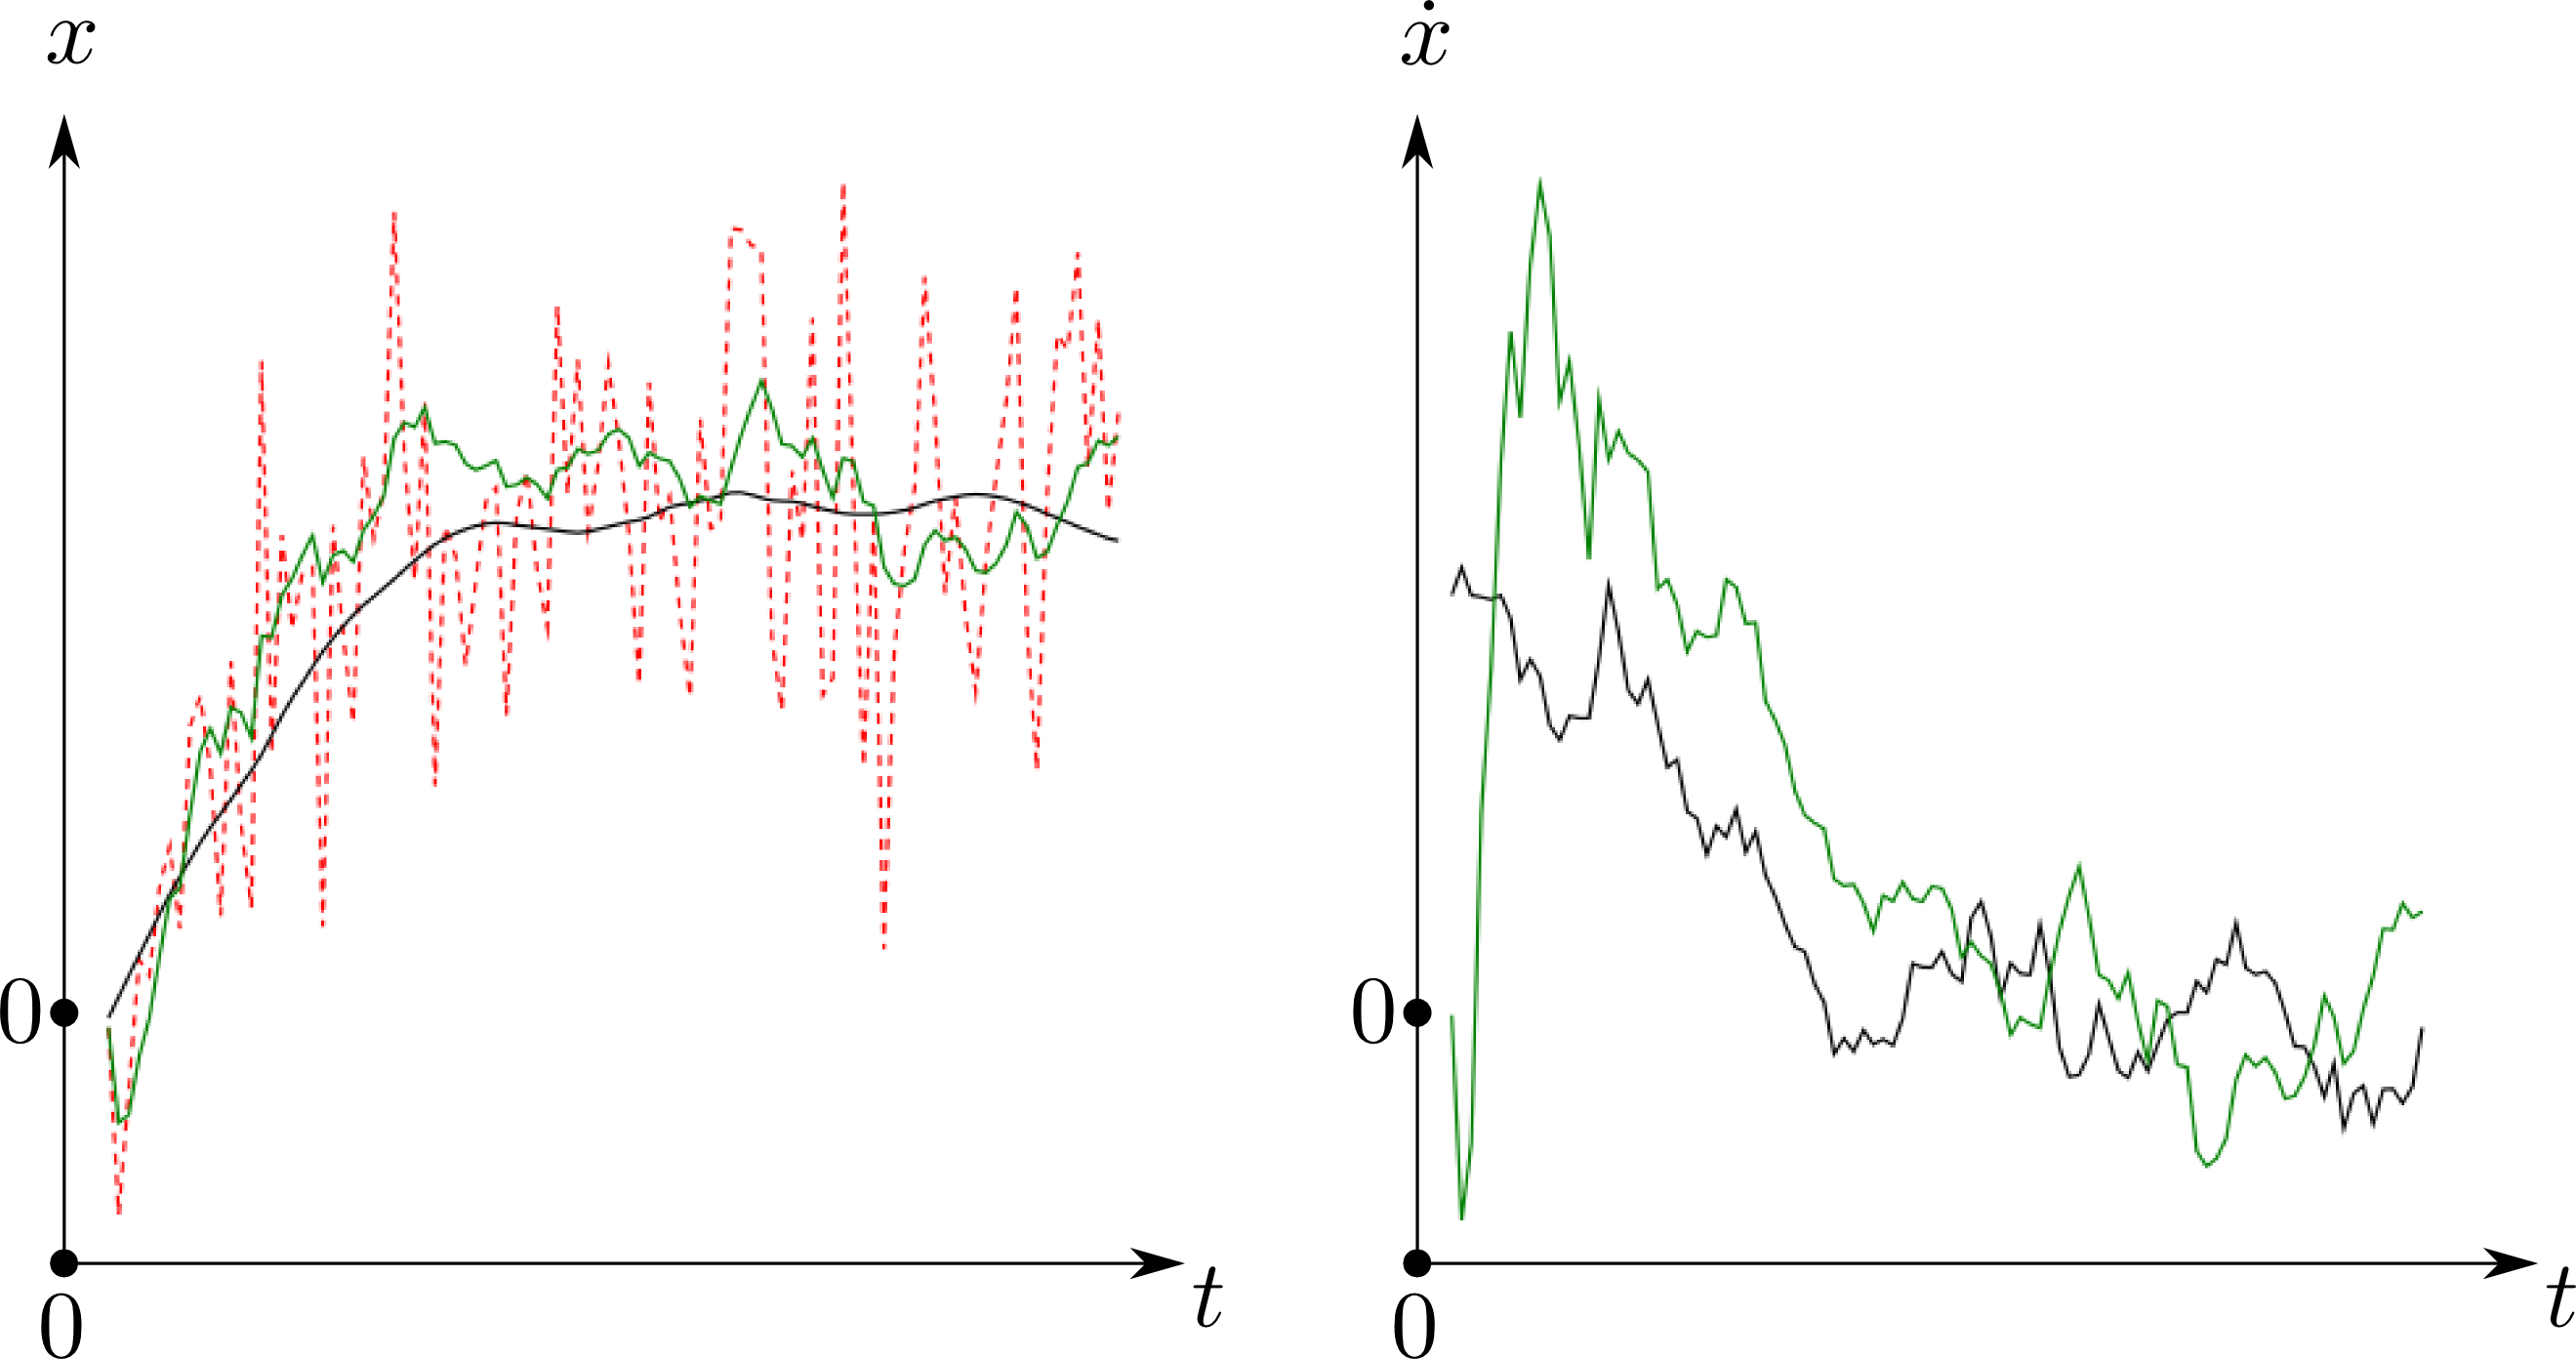
\includegraphics[width=0.7\textwidth]{Kalman.png} 
    \caption{Kalman's Filter: $\crule[red]{0.4cm}{0.4cm}$ Observed data; $\crule[ForestGreen]{0.4cm}{0.4cm}$ Filtered process; $\crule{0.4cm}{0.4cm}$ Real data \cite{wiki:Kalman_filter}.}
    \label{fig:kalman}
\end{figure}

From the mathematical viewpoint, we need to make sense of this kind of equations, since with the usual tools of calculus, it is not possible to treat them. Our goal then, in this work, is to give the foundations that allow us to treat this equations. In particular, firstly we're going to define the Itô's Integral and then we'll be ready to tackle stochastic differential equations.

\newpage
\section{Stochastic Integrals}

\subsection{Formalizing the `noise'}

To study the equation \eqref{eq:sde}, the first step is to give a formalization for the `noise' that we are going to consider. In our case, we'll consider the `white noise', which is a generalized stochastic process $W_t$ with gaussian probability distribution with mean zero, finite variance such that $\mathbb{E}[W_sW_t]=0$ whenever $t\neq s$.

In other words, the `noise' will be represented by some stochastic process $W_t$ and our goal is to satisfy the following properties:
\begin{itemize}
	\item If $t_1 \neq t_2$, then $W_{t_1}$ and $W_{t_2}$ are independent.
	\item The collection $\{W_t\}$ is stationary, i.e., the joint distribution of any collections of $W_t$ does not depend on $t$.
	\item $\mathbb{E}[W_t] = 0$ for all $t$.
\end{itemize}

However, this process $W_t$ does not have reasonable properties (does not have continuous paths, and it is not measurable for finite time). So our first goal is to replace $W_t$ with some convenient stochastic process.

Let $0 = t_0 < t_1 < \ldots < t_m = t$ and consider the discrete version
\[
	X_{k+1} - X_k = b(t_k,X_k)\Delta t_k + \sigma(t_k,X_k)W_k \Delta t_k
\]

Now, replace $W_k \Delta t_k = \Delta V_k = V_{k+1} - V_k$, where $V_t$ is a stochastic process. Since we want $V_t$ to have stationary independent increments with mean zero, the only suitable process with continuous paths is the Brownian motion, represented in the Figure \ref{fig:brownian_motion}.

Hence, we take $V_t = B_t$, thus obtaining
\[
	X_k = X_0 + \sum_{j=0}^{k-1} b(t_j, X_j) \Delta t_j + \sum_{j=0}^{k-1} \sigma(t_j, X_j) \Delta B_j
\]

Taking the limit as $\Delta t_j$ goes to zero, we have
\[
	X_k = X_0 + \int_0^t b(s, X_s) \, \mathrm{d}s + \int_0^t \sigma(s, X_s) \, \mathrm{d}B_s
\]

Notice that
\[
B_t-B_s=W_s(t-s)
\]
for all $t\geq s$, i.e., the `white noise' is the derivative, with respect to time, of the Brownian motion.

\begin{figure}[h!]
\centering
\pgfmathsetseed{3}
\begin{tikzpicture}[scale=1.2]
  \begin{axis}
    \addplot table [
        brownian motion = {%
        	start = 0,	
            max =  0.5,
            min = -0.75
        }
    ] {\loadedtable};
    \addplot table [
        brownian motion = {%
            start =  0,
            min   = -0.5,
            max   =  0.75
        }
    ] {\loadedtable};
  \end{axis}
\end{tikzpicture}
\caption{Two realizations of the Brownian motion \cite{texexchange:brownian-tikz}}
\label{fig:brownian_motion}
\end{figure}

\subsection{Preparing the Terrain}

Now we can start treating the equation. In order to do that, notice that in the determinist case, in which there isn't a `noise', we have an equation of the form
\begin{equation}
	\frac{\, \mathrm{d} X_t}{\, \mathrm{d} t} = b(t, X_t), \quad X_0 = x_0
\end{equation}

In this case, a solution is a function $X_t$ such that
\begin{equation}
	X_t - X_0 = \int_0^T b(s, X_s) \, \mathrm{d}s
\end{equation}
This function can be understood as a stochastic process over a space of probability given by a single point.

Using the formalism above, we propose as a solution to the equation \eqref{eq:sde} an identity of the form
\begin{equation}\label{eq:sde-sol-prop}
	X_t - X_0 = \int_0^t b(s, X_s) \, \mathrm{d}s + \int_0^t \sigma(s, X_s) \, \mathrm{d}B_s
\end{equation}
where the left integral is a Lebesgue-Stieltjes' integral, but the right integral is what still needs to be formalized. 

As said earlier, our task is to understand the following integral
\begin{equation}\label{eq:gen_ito_integrand}
	\int_S^T f(t, \omega) \, \mathrm{d}B_t(\omega)
\end{equation}
where $f : [0, \infty] \times \Omega \longrightarrow \textbf{R}$.

The idea will be the following: we'll first define the integral for the most elementary functions and, after that, using approximations and convergence criteria, we'll define it for the other classes of functions.

Since it is natural to approximate a given function $f(t, \omega)$ by
\[
	\sum_j f(t_j^\ast, \omega) \chi_{[t_j, t_{j+1})}(t)
\]
where $t_j^\ast \in [t_j, t_{j+1}]$, we could define the integral \eqref{eq:gen_ito_integrand} as follows
\[
	\int_S^T f(t, \omega) \, \mathrm{d}B_t(\omega) = \lim_{n \to \infty} f(t_j^\ast,\omega) [B_{t_{j+1}} - B_{t_j}](\omega)
\]

However, the choice of points $t_j^\ast$ make a difference here. If we take $t_j^\ast = t_j$, the left end point, then we obtain the \textbf{Itô integral}, denoted by
\[
	\int_S^T f(t, \omega) \, \mathrm{d}B_t(\omega)
\]

If, on the other hand, we take $t_j^\ast = (t_j + t_{j+1})/2$, the mid point, then we obtain the \textbf{Stratonovich integral}, denoted by
\[
	\int_S^T f(t, \omega) \circ \, \mathrm{d}B_t(\omega)
\]

One of the advantages of Itô integral is its application in Finance. Intuitively, by taking the leftmost point, one does not have to know the future, like whether a stock goes up or down.

Related to this intuition, and developing the Ito integral, we must restrict ourselves to functions $f$ that only depends on the behaviour of $B_s(\omega)$ up to the time $t_j$. 

\begin{definition}
	Let $B_t(\omega)$ be a Brownian motion. We define $\mathfrak{F}_t$ as the $\sigma$-algebra generated by the random variables $B_s$, where $s \leq t$. I.e., $\mathfrak{F}_t$ is the smallest $\sigma$-algebra containing all sets
	\[
		\{ \omega : B_{t_1}(\omega) \in F_1, \ldots, B_{t_k}(\omega) \} \in F_k
	\]
	where $t_j \leq t$ and $F_j \subseteq \textbf{R}^n$ are Borel sets, $j \leq k = 1, 2, \ldots$.
\end{definition}

The intuition behind this definition is that $\mathfrak{F}_t$ can be thought as the `history of $B_s$ up to the time $t$'. A function $h(\omega)$ is $\mathfrak{F}_t$-measurable if $h$ depends only on the values from $B_0$ up to $B_t$. I.e., it does not depend on the `future'. 

\begin{definition}[$\mathfrak{N}_t$-Adapted]
	Let $\{ \mathfrak{N}_t \}_{t \geq 0}$ be an increasing family of $\sigma$-algebras of subsets of $\Omega$. A process $g(t,\omega) : [0, \infty) \times \Omega \longrightarrow \textbf{R}^n$ is \textbf{$\mathfrak{N}_t$-adapted} if for each $t \geq 0$ the function $\omega \longrightarrow g(t,\omega)$ is $\mathfrak{N}_t$-measurable.
\end{definition}

\begin{example}
	The process $h_1(t, \omega) = B_{t/2}(\omega)$ is $\mathfrak{F}_t$-measurable and, hence, $\mathfrak{F}_t$-adapted. Notice that this process only depends on previous information.
	
	However, the process $h_2(t, \omega) = B_{2t}(\omega)$ is not $\mathfrak{F}_t$-measurable and, hence, it is not $\mathfrak{F}_t$-adapted. That's because the process $h_2$ depends on future information.
\end{example}

%Example. Let $T > 0$, and $\Delta (t) = \max_{t < s < T} \{ X_s \}$ is not adapted to $X_t$.
%
%If $B_t \sim N(0,t)$ and $X_t = \sigma B)t \sim N(0, \sigma^2 t)$ and $\int \sigma \, \mathrm{d}B_t$.
%
%If $\Delta(t)$ is a process depending only on $t$, then 
%\[
%	X(t) = \int \Delta(t) \, \mathrm{d}B_t
%\]
%has Normal distribution at all time.

\subsection{Constructing the Itô Integral}

The class of functions for which the Itô integral will be first defined is the following.

\begin{definition}\label{def:ito-class}
	Let $\mathfrak{V}(S,T)$ be the class of functions
	\[
		f(t, \omega) : [0, \infty) \times \Omega \longrightarrow \textbf{R}
	\]
	such that
	\begin{enumerate}
		\item The function $(t, \omega) \longrightarrow f(t, \omega)$ is $\mathfrak{B} \times \mathfrak{F}$-measurable, where $\mathfrak{B}$ denotes the Borel $\sigma$-algebra on $[0, \infty)$.
		\item The function $f(t,\omega)$ is $\mathfrak{F}_t$-adapted.
		\item $\mathbb{E} \left[ \int_S^T f(t, \omega)^2 \, \mathrm{d}t \right] < \infty$.
	\end{enumerate}
\end{definition}

Given functions $f \in \mathfrak{V}$, in order to define the Ito integral
\[
	I[f](\omega) = \int_S^T f(t, \omega)\, \mathrm{d}B_t(\omega)
\]
we are going to define $I[\varphi]$ for a simple class of functions $\varphi$ and then show how each $f \in \mathfrak{V}$ can be approximated by $\varphi$.

\begin{definition}[Elementary functions]
	A function $\varphi \in \mathfrak{V}$ is \textbf{elementary} if it has the form
\[
	\varphi(t, \omega) = \sum_j e_j(\omega) \chi_{[t_j, t_{j+1})}(t)
\]
\end{definition}

Since $\varphi \in \mathfrak{V}$, each function $e_j$ is $\mathfrak{F}_j$-measurable. And, as we did before, we define
\[
	\int_S^T \varphi (t, \omega) \, \mathrm{d}B_t(\omega) = \sum_{j \geq 0} e_j(\omega) [B_{j+1} - B_j](\omega)
\]

To further our development of the Ito integral, we need the following result.

\begin{theorem}[Itô isometry]
	If $\varphi(t, \omega)$ is bounded and elementary, then
	\[
		\mathbb{E}\left[\left( \int_S^T \varphi(t,\omega) \, \mathrm{d}B_t(\omega) \right)^2 \right] = \mathbb{E} \left[\int_S^T \varphi(t,\omega)^2 \, \mathrm{d}t \right]
	\]
\end{theorem}

Using this isometry, it is possible to extended the previous definition to functions in $\mathfrak{V}$ by the following steps.

\begin{enumerate}
	\item Let $g(\omega) \in \mathfrak{V}$ be bounded and continuous for each $\omega$. Then there exists elementary functions $\varphi_n \in \mathfrak{V}$ such that
	\[
		\mathbb{E} \left[ \int_S^T (g-\varphi_n)^2 \, \mathrm{d}t \right] \longrightarrow 0
	\]
	as $n \to \infty$.
	\item Let $h \in \mathfrak{V}$ be bounded, then there exists bounded functions $g_n \in \mathfrak{V}$ such that $g_n (\omega)$ are continuous for all $\omega$ and $n$, and
	\[
		\mathbb{E} \left[ \int_S^T (h-g_n)^2 \, \mathrm{d}t \right] \longrightarrow 0
	\]
	\item Let $f \in \mathfrak{V}$. Then there exists a sequence of functions $(h_n) \subseteq \mathfrak{V}$ such that $h_n$ is bounded for each $n$ and 
	\[
		\mathbb{E} \left[ \int_S^T (f-h_n)^2 \, \mathrm{d}t \right] \longrightarrow 0
	\]
	as $n \to \infty$.
\end{enumerate}

Please note that we started from bounded and continuous functions, generalized into bounded functions and then generalized further into any function in our class $\mathfrak{V}$.

These steps can be summarized in the following result, which guarantees that the elementary functions are dense in $\mathfrak{V}(S,T)$.

\begin{theorem}
If $g\in \mathfrak{V}(S,T)$, then there exists a sequence of elementary functions $\varphi_n\in \mathfrak{V}(S,T)$ such that $\varphi_n\to g$ in $L^2(P)$
\end{theorem}

Finally, we can define the Itô integral as follows.

\begin{definition}[The Itô integral]
	Let $f \in \mathfrak{V}(S,T)$, then the \textbf{Itô integral} of $f$, from $S$ to $T$ is
	\[
		\int_S^T f(t, \omega) \, \mathrm{d}B_t(\omega) = \lim_{n \to \infty} \int_S^T \varphi_n (t, \omega)  \, \mathrm{d}B_t(\omega)
	\]
	where the limit is in $L^2(P)$ and $(\varphi_n)$ is a sequence of elementary functions such that
	\[
		\mathbb{E} \left[ \int_S^T (f(t, \omega) - \varphi_n(t, \omega))^2 \, \mathrm{d}t \right] \longrightarrow 0
	\] 
	as $n \to \infty$.
\end{definition}

This new definition induces a generalized form of the Ito isometry.

\begin{theorem}[Ito isometry]
	For all $f \in \mathfrak{V}(S,T)$,	
	\[
		\mathbb{E}\left[\left( \int_S^T f(t,\omega) \, \mathrm{d}B_t(\omega) \right)^2 \right] = \mathbb{E} \left[\int_S^T f(t,\omega)^2 \, \mathrm{d}t \right]
	\]
\end{theorem}

\begin{corollary}
	If $f(t, \omega) \in \mathfrak{V}(S,T)$ and $f_n(t, \omega) \in \mathfrak{V}(S,T)$ and
	\[
		\mathbb{E}\left[\left( \int_S^T f_n(t,\omega) - f(t, \omega) \right)^2 \, \mathrm{d}t \right] \longrightarrow 0
		\]
	as $n \to \infty$, then
	\[
		\int_S^T f_n(t, \omega) \, \mathrm{d}B_t(\omega) \longrightarrow \int_S^T f(t, \omega) \, \mathrm{d} B)t(\omega)
	\]
	in $L^2(P)$ as $n \to \infty$.
\end{corollary}

\begin{example}
	We wish to compute the integral
	\[
		\int_0^T B(t) \, \mathrm{d}B(t)
	\]
	
	\textbf{Step 1.} Let
	\[
		\varphi_n(t) = \sum_{i=0}^{n-1} B_n(t_i^n)[B_n(t_{i+1}^n) - B_n(t_i^n)]
	\]
	be a sequence of elementary functions. Then,
	\begin{equation*}
		\begin{aligned}
			\mathbb{E} \left[ \int_0^T (\varphi_n - B_s)^2 ~\mathrm{d}s \right]
			&= \mathbb{E} \left[ \sum_j \int_{t_j}^{t_{j+1}} (B_j - B_s)^2 ~\mathrm{d}s \right]
			= \sum_j \int_{t_j}^{t_{j+1}} (s - t_j)^2 ~\mathrm{d}s \\
			&= \sum_j \frac{1}{2} \left(t_{j+1} - t_j \right)^2 \longrightarrow 0 \, \text{ when } \Delta t_j \to 0
		\end{aligned}
	\end{equation*}
	I.e., $\varphi_n(t)$ converges to $B(t)$ almost surely as $\max_i (t_{i+1}^n - t_i^n) \to 0$ by the continuity of $B(t)$.
	
	\textbf{Step 2.} Now notice that
	\begin{equation*}
		\begin{aligned}
			B_n(t_i)[B_n(t_{i+1}) - B_n(t_i)] &= B_n(t_{i+1}) B_n(t_i) - B_n^2(t_i) + B_n^2(t_{i+1}) - B_n^2(t_{i+1}) \\
			&= \frac{1}{2} [B_n^2(t_{i+1}) - B_n^2(t_i) - (B_n(t_{i+1}) - B_n(t_i))^2 ]
		\end{aligned}
	\end{equation*}
	
	\textbf{Step 3.} With these two results, we can write the original integral as
	\[
		\int_0^T X_n(t) \, \mathrm{d}B(t) = \frac{1}{2} \sum_{i=0}^{n-1} \left[ B_n^2(t_{i+1}) - B_n^2(t_i) \right] - \frac{1}{2} \sum_{i=0}^{n-1} \left[ B_n(t_{i+1}) - B_n(t_i) \right]^2
	\]
	
	\textbf{Step 4.} Since the first sum is a telescopic sum and the second one converges in probability to $T$ by the quadratic variation of Brownian motion, we have
	\[
		\int_0^T X_n(t) \, \mathrm{d}B(t) = \frac{1}{2} B^2(t) - \frac{1}{2} B^2(0) - \frac{1}{2}T = \frac{1}{2} B^2(t) - \frac{1}{2}T 
	\]
	
	Hence, the integral converges in $L^2(P)$ to
	\[
		\int_0^T B(t) \, \mathrm{d}B(t) = \lim_{n \to \infty} \int_0^T X_n(t) \, \mathrm{d}B(t) = \frac{1}{2} B^2(t) - \frac{1}{2}T 
	\]
\end{example}

\subsection{Properties} % Shreve p. 148

Before heading to more theoretical and important results, let us notice some natural facts of the Itô integral.

\begin{theorem}
	Let $f, g \in \mathfrak{V}(0,T)$ and let $0 \leq S < U < T$. Then
	\begin{enumerate}
		\item $\int_S^T f \, \mathrm{d}B_t = \int_S^U f \, \mathrm{d}B_t + \int_U^T f \, \mathrm{d}B_t$ for a.a. $\omega$.
		\item $\int_S^T (cf + g) \, \mathrm{d}B_t = c \int_S^T f \, \mathrm{d}B_t + \int_S^T g \, \mathrm{d}B_t$ where $c \in \textbf{R}$.
		\item $\mathbb{E} \left[ \int_S^T f \, \mathrm{d}B_t \right] = 0$.
		\item $\int_S^T f \, \mathrm{d}B_t$ is $\mathfrak{F}_T$-measurable.
	\end{enumerate}
\end{theorem}

With the Doob's martingale inequality, it can be proved that the Itô integral can be chosen to depend continuously on $t$. A proof of this fact is on the third chapter of \cite{oksendal2013stochastic}.

Now an important result is that the Itô integral is a martingale.

\begin{theorem}
	Let $f(t, \omega) \in \mathfrak{V}(0,T)$ for all $T$. Then
	\[
		M_t(\omega)  = \int_0^t f(s,\omega)\, \mathrm{d}B_s
	\]
	is a martingale w.r.t. $\mathfrak{F}_t$ and for $\lambda, T > 0$
	\[
		P \left[ \sup_{0 \leq t \leq T} |M_t| \geq \lambda \right] \leq \frac{1}{\lambda^2} \mathbb{E} \left[ \int_0^T f(s,\omega)^2 \, \mathrm{d}s \right]
	\]
\end{theorem}

Summarizing, the Itô integral is continuous, adapted, linear, a martingale, satisfies the Itô isometry and has Quadratic variation.

\subsection{Extensions}

Using the concept of martingales, we can generalize the Itô integral for a larger class of functions than $\mathfrak{V}$.

Considering the Definition \ref{def:ito-class}, we can relax the condition 2. into
\begin{itemize}
	\item[2.'] There exists an increasing familiy of $\sigma$-algebras $\mathfrak{H}_t$ such that $B_t$ is a martingale w.r.t. $\mathfrak{H}_t$ and $f_t$ is $\mathfrak{H}_t$-adapted.
\end{itemize}

The idea here is that $B_t$ must remain a martingale with respect to the history of $f_s$. 

Another way of extending the Itô integral definition is by weaking the condition 3. into
\begin{itemize}
	\item[3.'] $P \left[ \int_S^T f(s, \omega)^2 \, \mathrm{d}s < \infty \right] = 1$
\end{itemize}

Too understand why this works, let $\mathfrak{W}_{\mathfrak{H}} (S,T)$ denote the class of processes satisfying conditions 1, 2' and 3' above. Then, in the 1-dimensional Brownian motion, for all $t$ there exists step functions $f_n \in \mathfrak{W}_{\mathfrak{H}}$ such that
\[
	\int_0^t |f_n - f|^2 \, \mathrm{d}s \longrightarrow 0
\]
in probability.

Now, since $\int_0^t f_n(s, \omega) \, \mathrm{d}B_s(\omega)$ converges in probability to a random variable and the limit depends only on $f$, we define
\[
	\int_0^t f(s, \omega) \, \mathrm{d}B_s(\omega) = \lim_{n \to \infty} \int_0^t f_n(s, \omega) \, \mathrm{d}B_s(\omega)
\]
where the limit is in probability and $f \in \mathfrak{W}_{\mathfrak{H}}$.

\subsection{Stratonovich integral}

As we saw, the Itô integral is one possible interpretation of the integral 
\[
	\int_S^T f(t, \omega) \, \mathrm{d}B_t(\omega)
\]

The Stratonovich integral is another possibility and, in general, leads to different results (except when the integrating function has a derivative). In some cases, the Stratonovich definition may be adequate.

In other cases, Itô's feature of `not looking in the future' (as \cite{oksendal2013stochastic} puts it), justifies its use in biology and finance, for example. Moreover, Itô integral is a martingale, and Stratonovich's is not. This gives an important computational advantage to Itô's definition. 

And, to quote \cite{shreve2004stochastic},

\begin{quotation}
	However, it [Stratonovich's integral] is inappropriate for finance. In finance, the integrand represents a position in an asset and the integrator represents the price of that asset. We cannot decide at 1:00 p.m. which position we took at 9:00 a.m. We must decide the position at the beginning of each time interval, and the Ito integral is the limit of the gain achieved by that kind of trading as the time between trades approaches zero.
\end{quotation}

However, Stratonovich integral is used in manifolds and is of particular interest to physicists for obeying rules of classical calculus, such as the chain rule.

% DRAFTS

%\begin{theorem}
%	If $g(t, B_t)$ is adapted to $B_t$, then
%	\[
%		\int g(t,B_t) \, \mathrm{d}B_t
%	\]
%	is a martingale as long as $g$ is `reasonable'.
%\end{theorem}
%
%If a SDE has a drift term, then it is not a martingale. If it doesn't, then it is a martingale.

%Differential form of the quadratic variation:
%	\[
%		(\, \mathrm{d}B_t)^2 = \, \mathrm{d}t
%	\]
%	
%Simple Ito's Lemma: $\, \mathrm{d} f = f'(B_t)dB_t + 1/2 f''(B_t)\, \mathrm{d}t$
%
%Ito's Lemma: if $f$ is smooth function, $X_t : \, \mathrm{d}X_t = \mu \, \mathrm{d}t + \sigma \, \mathrm{d}B_t$, then
%\[
%	\, \mathrm{d} f(t, X_t) = \left( \frac{\partial f}{\partial t} + \mu \frac{\partial f}{\partial x} + \frac{1}{2} \sigma^2 \frac{\partial^2 f}{\partial x^2} \right) \, \mathrm{d}t + \sigma \frac{\partial f}{\partial x} \, \mathrm{d}B_t
%\]
%
%Proof: take Taylor expansion.
%
%Example:
%
%If $f(X) = X^2$, then 
%\[
%	\, \mathrm{d}f(B_t) = 2 B_t \, \mathrm{d} B_t + \frac{1}{2} 2 \, \mathrm{d}t
%\]
%because $\frac{\partial f}{\partial t} = 0$, $\frac{\partial f}{\partial x} = 2x$, $\frac{\partial^2 f}{\partial x^2} = 2$, $\mu = 0$, and $\sigma = 1$.
%
%Another way:
%\[
%	\, \mathrm{d}f(B_t) = \frac{\partial f}{\partial t} \, \mathrm{d}t + \frac{\partial f}{\partial x} \, \mathrm{d}B_t + \frac{1}{2} \frac{\partial^2 f}{\partial x^2} (\, \mathrm{d}B_t)^2 = 2 B_t \, \mathrm{d} B_t + \, \mathrm{d} t
%\]
%
%Example:
%
%If $f(t,X) = e^{\mu t + \sigma X}$, then
%\begin{equation*}
%\begin{aligned}
%	\, \mathrm{d}f(t, B_t) &= \frac{\partial f}{\partial t} \, \mathrm{d}t + \frac{\partial f}{\partial x} \, \mathrm{d}B_t + \frac{1}{2} \frac{\partial^2 f}{\partial x^2} (\, \mathrm{d}B_t)^2 \\
%	&= \mu e^{\mu t + \sigma x}\, \mathrm{d}t + \sigma e^{\mu t + \sigma x} \, \mathrm{d}B_t + \frac{1}{2} \sigma^2 e^{\mu t + \sigma x} \, \mathrm{d}t \\
%	&= \left( \mu + \frac{1}{2} \sigma^2 \right) f \, \mathrm{d}t + \sigma f \, \mathrm{d}B_t
%\end{aligned}
%\end{equation*}
%
%Integral Definition:
%\[
%	F(t, B_t) = \int f(t, B_t) \, \mathrm{d}B_t + \int g(t, B_t) \, \mathrm{d}t
%\]
%if
%\[
%	\, \mathrm{d}F = f \, \mathrm{d}B_t + g \, \mathrm{d}t
%\]

In this section, we presented a formalism for modeling evolution process with noise using the Brownian motion. We saw that the classical notion of solution doesn't work and we proposed a new interpretation. As a result, it was necessary to construct a new theory of integration and, with that, the Itô and Stratonovich integrals. We hence studied the properties of these integrals.

Given that, we can advance on more elaborated questions, for example: does the equation \eqref{eq:sde} has a solution? Under which hypothesis? How can we study the behavior of the solution?

\newpage
\section{The Ito Formula and the Martingale Representation Theorem} % Shreve 157 (p.137)

% October-January

\newpage
\section{Stochastic Differential Equations}

% February-May

\appendix

\newpage
\section{Measure Theory}

\subsection{Measurable Spaces}

Given a set $S$, on what collection $\mathfrak{S}$ of subsets of $S$ are suitable to be a domain of measure?

\begin{definition}
	Let $S$ be a set and $\mathfrak{S}$ be a family of subsets of $S$. Then $\mathfrak{S}$ is called a \textbf{$\sigma$-algebra} on $S$ if
	\begin{enumerate}
		\item $\emptyset, S \in \mathfrak{S}$.
		\item If $A \in \mathfrak{S}$, then $A^c \in \mathfrak{S}$.
		\item If $A_1, A_2, \ldots \in \mathfrak{S}$, then $\bigcup_{i=1}^\infty A_i \in \mathfrak{S}$.
	\end{enumerate}

	The pair $(S, \mathfrak{S})$ is said to be a \textbf{measurable space}, and any subset $A \subseteq \mathfrak{S}$ is called an \textbf{$\mathfrak{S}$-measurable set}.
\end{definition}

For any set $S$ and any collection $\mathfrak{A}$ of subsets of $S$ there is at least one $\sigma$-algebra containing $\mathfrak{A}$: the family of all subsets of $S$. Taking the intersection of all the $\sigma$-algebras containing $\mathfrak{A}$, we obtain the smallest $\sigma$-algebra containing $\mathfrak{A}$, which is called the \textbf{$\sigma$-algebra generated by $\mathfrak{A}$}.

Particularlly, the smallest $\sigma$-algebra containing all of the open sets of $\textbf{R}$ is called the \textbf{Boreal algebra} for $\textbf{R}$ and is denoted by $\mathfrak{B}$. Any set in $\mathfrak{B}$ is called a \textbf{Borel set}.

\subsection{Measures}

Now, how can we assign a size (or a probability) to all the sets in $\mathfrak{S}$?

\begin{definition}
	Let $(S, \mathfrak{S})$ be a measurable space. A \textbf{measure} is an extended real-valued function $\mu : \mathfrak{S} \longrightarrow \overline{\textbf{R}}$ such that 
	\begin{enumerate}
		\item $\mu ( \emptyset ) = 0$;
		\item $\mu(A) \geq 0$, for all $A \in \mathfrak{S}$;
		\item If $(A_n)_{n=1}^\infty$ is a countable, disjoint sequence of subsets in $\mathfrak{S}$, then $\mu(\bigcup_{n=1}^\infty A_n) = \sum_{n=1}^\infty \mu(A_n)$.
	\end{enumerate}

	The triple $(S, \mathfrak{S}, \mu)$ is called a \textbf{measure space}.
\end{definition}

A measure is nonnegative, assigns zero to the null set, and is \textbf{countably additive}. If $\mu(S) < \infty$, then $\mu$ is finite.

We say that a proposition holds \textbf{almost everywhere (a.e.)} if there exists a set $A \in \mathfrak{S}$ with $\mu(A) = 0$, such that the proposition holds on the complement of $A$. Intuitively, the proposition holds everywhere except on sets of measure zero.

For example, a sequence of functions $(f_n)$ on $S$ converges a.e. to a function $f$ if there exists $A \in \mathfrak{S}$ with $\mu(A) = 0$ such that $\lim_{n \to \infty} f_n(x) = f(x)$ for all $x \in A^c$.

If $\mu(S) = 1$, then $\mu$ is a \textbf{probability measure} and $(S, \mathfrak{S}, \mu)$ is called a \textbf{probability space}. Any measurable set $A \in \mathfrak{S}$ is called and \textbf{event} and $\mu(A)$ is the \textbf{probability of the event $A$}. In a probability space, the phrase \textbf{almost surely (a.s.)} is used interchangeably with `almost everywhere'.

Notice that if $A, B \in \mathfrak{S}$ and $A \subseteq B$, then $\mu(A) \leq \mu(B)$. If $\mu(A) < \infty$, then $\mu(B \setminus A) = \mu(B) - \mu(A)$.

\begin{theorem}
	Let $(S, \mathfrak{S}, \mu)$ be a measure space.
	\begin{enumerate}
		\item If $(A_n)_{n=1}^\infty$ is an increasing sequence in $\mathfrak{S}$ (i.e. if $A_n \subseteq A_{n+1}$ for all $n$), then \[ \mu \left( \bigcup_{n=1}^\infty A_n \right) = \lim_{n \to \infty} \mu(A_n) \] 
		\item If $(B_n)_{n=1}^\infty$ is a decreasing sequence in $\mathfrak{S}$ (i.e. if $B_{n+1} \subseteq B_n$ for all $n$) and if $\mu(B_m) < \infty$ for some $m$, then \[ \mu \left( \bigcap_{n=1}^\infty B_n \right) = \lim_{n \to \infty} \mu(B_n) \] 
	\end{enumerate}
\end{theorem}

First, we define a measure on a small family of sets and then present an extension theorem.

\begin{definition}
	Let $S$ be a set and $\mathfrak{A}$ be a family of subsets of $S$. Then $\mathfrak{A}$ is called an \textbf{algebra} if 
	\begin{enumerate}
		\item $\emptyset, S \in \mathfrak{A}$;
		\item $A \in \mathfrak{A}$ implies $A^c \in \mathfrak{A}$;
		\item $A_1, A_2, \ldots, A_n \in \mathfrak{A}$ implies $\bigcup_{i=1}^n A_i \in \mathfrak{A}$.
	\end{enumerate}
\end{definition}

I.e., an algebra is closed under complementation and finite union. On an algebra, the idea of measure is very much similar to the definition on a $\sigma$-algebra.

\begin{definition}
	Let $S$ be a set, and let $\mathfrak{A}$ be an algebra of subsets of $S$. A \textbf{measure} is a real-valued function $\mu : \mathfrak{A} \longrightarrow \overline{\textbf{R}}$ such that 
	\begin{enumerate}
		\item $\mu ( \emptyset ) = 0$;
		\item $\mu(A) \geq 0$, for all $A \in \mathfrak{A}$;
		\item If $(A_n)_{n=1}^\infty$ is a disjoint sequence of sets in $\mathfrak{A}$ with $\bigcup_{n=1}^\infty A_n \in \mathfrak{A}$, then $\mu \left( \bigcup_{n=1}^\infty A_n \right) = \sum_{n=1}^\infty \mu(A_n)$.
	\end{enumerate}
\end{definition}

Notice that last item is different from the definition on a $\sigma$-algebra. Here, we require that the union is contained in the algebra.

Although it is easier to define measures on algebras, it is more convenient to work with $\sigma$-algebras.

\begin{theorem}[Caratheodory Extension Theorem]\label{thm:caratheodory}
	Let $S$ be a set, $\mathfrak{A}$ an algebra of its subsets, and $\mu$ a measure on $\mathfrak{A}$. Let $\mathfrak{S}$ be the smallest $\sigma$-algebra containing $\mathfrak{A}$. Then there exists a measure $\mu^{\ast}$ on $\mathfrak{S}$ such that $\mu(A) = \mu^{\ast}(A)$, for all $A \in \mathfrak{A}$.
\end{theorem}

To rule out the possibility of more than one extension of $\mu$ to $\mathfrak{S}$, we'll need the following definition

\begin{definition}
	Let $S$ be a set, $\mathfrak{A}$ an algebra of its subsets, and $\mu$ a measure on $\mathfrak{A}$. If there is a countable sequence of sets $(A_i)_{i=1}^\infty \in \mathfrak{A}$ with $\mu(A_i) < \infty$ for all $i$, and $S = \bigcup_{i=1}^\infty A_i$, then $\mu$ is called \textbf{$\sigma$-finite}.
\end{definition}

By definition, any probability measure is $\sigma$-finite. And the next theorem shows that the extension of a $\sigma$-finite measure is unique.

\begin{theorem}[Hahn Extension Theorem]
	Let $S$, $\mathfrak{A}$, $\mu$ and $\mathfrak{S}$ be as specified in \hyperref[thm:caratheodory]{Caratheodory Extension Theorem}. If $\mu$ is $\sigma$-finite, then the extension $\mu^{\ast}$ to $\mathfrak{S}$ is unique.
\end{theorem}

\begin{definition}
	Let $(S, \mathfrak{S}, \mu)$ be a measure space, $A \in \mathfrak{S}$ be any set with measure zero, and let $C \subseteq A$. Denoting by $\mathfrak{C}$ the family of such sets $C$, i.e.,
	\[
		\mathfrak{C} = \{ C \subset S : C \subseteq A \text{ for some } A \in \mathfrak{S} \text{ with } \mu(A) = 0 \}
	\]

	The \textbf{completion} of $\mathfrak{S}$ is the family $\mathfrak{S}'$ constructed by starting with any set $B \in \mathfrak{S}$, and then adding and subtracting from it sets in $\mathfrak{C}$. That is 
	\[
		\mathfrak{S}' = \{ B' \subseteq S : B' = (B \cup C_1) \setminus C_2, \, B \in \mathfrak{S}, \, C_1, C_2 \in \mathfrak{C} \} 
	\]
\end{definition}

Intuitively, $\mathfrak{S}'$ consists of all the subsetes of $S$ that differ from a set in $\mathfrak{S}$ by a setset of a set of $\mu$-measure zero. Using this definition, a measure $\mu$ on $(S, \mathfrak{S})$ can be extended to $(S, \mathfrak{S}')$.

\subsection{Measurable Functions}

\begin{definition}
	Given a measurable space $(S, \mathfrak{S})$, a real-valued function $f : S \longrightarrow \textbf{R}$ is \textbf{measurable with respect to $\mathfrak{S}$} (or \textbf{$\mathfrak{S}$-measurable}) if 
	\[
		\{ s \in S : f(s) \leq a \} \in \mathfrak{S}, \, \forall a \in \textbf{R}
	\]
\end{definition}

If the space is a probability space, then $f$ is called a \textbf{random variable}.

Some cases in which measurability can be easily verified:
\begin{itemize}
	\item Any monotone or continuous function $f : \textbf{R} \longrightarrow \textbf{R}$ is measurable with respect to Borel sets.
	\item If $S$ is a countable set and $\mathfrak{S}$ is a complete $\sigma$-algebra for $S$ (i.e. contains all subsets of $S$), then all functions $f : S \longrightarrow \textbf{R}$ are $\mathfrak{S}$-measurable.
\end{itemize}

In more general cases, the measurability of a function is established by showing that it is the limit of a sequence of `simpler' functions. We'll do this progressively.

First, let $(S, \mathfrak{S})$ be a measurable space and consider the indicator function $\chi_A : S \longrightarrow \textbf{R}$ of the from
\[
\chi_A (s) = \begin{cases}
	1, & \text{if } s \in A\\
	0, & \text{if } s \notin A
	\end{cases}
\]
Clearly, $\chi_A$ is $\mathfrak{S}$-measurable iff. $A \in \mathfrak{S}$.

Now, consider the finite weighted sums of indicator functions:
\[
	\varphi(s) = \sum_{i=1}^n a_i \chi_{A_i}(s)
\]
where $(A_i)_{i=1}^n$ is a sequence of subsets of $S$, and $(a_i)_{i=1}^n$ is a sequence of real numbers. Functions like this are called \textbf{simple functions}.

If the sets $(A_i)$ form a partition of $S$ and if all of the values $a_i$ are distinct, then the previous equation is the \textbf{standard representation} of the function. If this is the case, then $\varphi$ is measurable iff. each $A_i \in \mathfrak{S}$.

As we'll see in the next two theorems, the set of all measurable functions consists of those that are pointwise limits of measurable simple functions.

First, any function $f$ that is pointwise limit of a sequence $(f_n)$ of measurable function is itself measurable.

\begin{theorem}[Pointwise convergence preserves measurability]
	Let $(S, \mathfrak{S})$ be a measurable space, and let $(f_n)$ be a sequence of $\mathfrak{S}$-measurable functions converging pointwise to $f$, i.e.,
	\[
		\lim_{n \to \infty} f_n(s) = f(s), \, \forall s \in S
	\]

	Then $f$ is also $\mathfrak{S}$-measurable.
\end{theorem}

Second, any measurable function $f$ can be expressed as the pointwise limit of a sequence $(\varphi_n)$ of measurable simple functions. If $f$ is nonnegative, the sequence can be chosen to be strictly increasing. And if $f$ is bounded, the sequence can be chosen to converge uniformly.

The idea is that we can construct a class of measurable functions by taking the class of measurable simple function and then closing this under pointwise convergence. The next result shows that this set contains all the measurable functions.

\begin{theorem}[Approximation of measurable functions by simple functions]
	Let $(S, \mathfrak{S})$ be a measurable space. If $f : S \longrightarrow \textbf{R}$ is $\mathfrak{S}$-measurable, then there exists a sequence of measurable simple functions $(\varphi_n)$ such that $\varphi_n \longrightarrow f$ pointwise. If $0 \leq f$, then the sequence can be chosen so that 
	\[
		0 \leq \varphi_n \leq \varphi_{n+1} \leq f
	\]
	for all $n$. If $f$ is bounded, then the sequence can be chosen so that $\varphi_n \longrightarrow f$ uniformly.
\end{theorem}

With these two theorems, we see that a function is measurable iff. it is the pointwise limit of a sequence of measurable simple functions. The standard way to prove that a function is measurable is to find such an approximation.

Some important properties follow. Suppose that $f$ and $g$ are $\mathfrak{S}$-measurable functions on $S$ and $c \in \textbf{R}$. Then,
\begin{itemize}
	\item The functions $f + g$, $f \cdot g$, $|f|$ and $c \cdot f$ are $\mathfrak{S}$-measurable.
	\item If $(f_n)$ is a sequence of $\mathfrak{S}$-measurable functions, then $\inf f_n$, $\sup f_n$, $\liminf f_n$ and $\limsup f_n$ are all $\mathfrak{S}$-measurable.
	\item All continuous functions on $\textbf{R}^l$ are $\mathfrak{B}^l$-measurable.
	\item The composition of Borel measurable functions are Borel measurable. However, this is not true for Lebesgue measurable functions.
\end{itemize}

\begin{definition}
	Let $(S, \mathfrak{S})$ and $(T, \mathfrak{T})$ be measurable spaces. Then the function $f : S \longrightarrow T$ is \textbf{measurable} if the inverse image of every measurable set is measurable, i.e., 
	\[
		\{ s \in S : f(s) \in A \} \in \mathfrak{S}, \, \forall A \in \mathfrak{T}
	\]
\end{definition}

Hence, if $(S, \mathfrak{S})$, $(T, \mathfrak{T})$, and $(U, \mathfrak{U})$ are measurable spaces, and $f : S \longrightarrow T$ and $g : T \longrightarrow U$ are measurable functions, then $h : S \longrightarrow U$ defined by $h(s) = g \circ f(s)$ is a measurable function.

\begin{definition}[Measurable selection]
	Let $(S, \mathfrak{S})$ and $(T, \mathfrak{T})$ be measurable spaces, and let $\Gamma$ be a correspondence of $S$ into $T$. Then the function $h : S \longrightarrow T$ is a \textbf{measurable selection from $\Gamma$} if $h$ is measurable and $h(s) \in \Gamma(s)$, for all $s \in S$.
\end{definition}

\begin{theorem}[Measurable Selection]
	Let $S \subseteq \textbf{R}^l$ and $T \subseteq \textbf{R}^m$ be Borel sets, with their Borel subsets $\mathfrak{S}$ and $\mathfrak{T}$. Let $\Gamma : S \longrightarrow T$ be a nonempty compact-valued and upper hemi-continuous (UHC) correspondence. Then there exists a measurable selection from $\Gamma$.
\end{theorem}

\subsection{Integration}

Let $(S, \mathfrak{S}, \mu)$ be a fixed measure space and $M(S, \mathfrak{S})$ be the space of measurable, extended real-valued functions on $S$. 

For a nonnegative, measurable and simple function, we have the following definition.

\begin{definition}
	Let $\varphi \in M^+(S, \mathfrak{S})$ be a measurable simple function, with the standard representation $\varphi(s) = \sum_{i=1}^n a_i \chi_{A_i}(s)$. Then the \textbf{integral of $\varphi$ with respect to $\mu$} is 
	\[
		\int_S \varphi(s) \, \mu(\mathrm{d} s) = \sum_{i=1}^n a_i \mu(A_i)
	\]
\end{definition}

To extended from simple functions to all $M^+(S, \mathfrak{S})$, we define

\begin{definition}
	For $f \in M^+(S, \mathfrak{S})$, the \textbf{integral of $f$ with respect to $\mu$} is 
	\[
		\int_A f(s) \, \mu(\mathrm{d}s) = \int_S f(s) \chi_A (s) \mu(\mathrm{d}s)
	\]
	We also denote the integrals above as $\int f \, \mathrm{d} \mu$ and $\int_A f \, \mathrm{d} \mu$. 
\end{definition}

Since any function $f \in M^+(S, \mathfrak{S})$ can be expressed as the limit of an increasing sequence $(\varphi_n)$ of simple functions in $M^+(S, \mathfrak{S})$. However, we cannot define the integral as the limit of such a sequence because it would leave open the possibility that the limit depends on the particular sequence chosen. The Monotone Convergence Theorem shows that the limit value is unique.

Before that, the following result shows that a simple function on a measure space can be used to define a new measure on the space.

\begin{lemma}
	If $\varphi \in M^+(S, \mathfrak{S})$ is a simple function and $\lambda: \mathfrak{S} \longrightarrow \textbf{R}$ is defined by
	\[
		\lambda(A) = \int_A \varphi\, \mathrm{d}\mu 
	\]
	for all $A \in \mathfrak{S}$, then $\lambda$ is a measure on $\mathfrak{S}$.
\end{lemma}

\begin{theorem}[Monotone Convergence Theorem]
	If $(f_n)$ is a monotone increasing sequence of functions in $M^+(S, \mathfrak{S})$ converging pointwise to $f$ then 
	\[
		\int f\, \mathrm{d}\mu = \lim_{n \to \infty} \int f_n \, \mathrm{d} \mu
	\]
\end{theorem}

Some important properties:

\begin{enumerate}
	\item If $f, g \in M^+(S, \mathfrak{S})$ and $c \geq 0$, then 
	\[
		\int (f+g)\, \mathrm{d}\mu = \int f\, \mathrm{d}\mu + \int g\, \mathrm{d}\mu
	\]
	and
	\[
		\int c\cdot f \, \mathrm{d}\mu = c \int f\, \mathrm{d}\mu
	\]
	\item If $f, g \in M^+(S, \mathfrak{S})$ and $f \leq g$, then
	\[
		\int f\, \mathrm{d}\mu \leq \int g\, \mathrm{d}\mu
	\]
	\item If $f \in M^+(S, \mathfrak{S})$ and $A, B \in \mathfrak{S}$ with $A \subseteq B$, then
	\[
		\int_A f\, \mathrm{d}\mu \leq \int_B f\, \mathrm{d}\mu
	\]
	\item If $f \in M^+(S, \mathfrak{S})$ and $A \in \mathfrak{S}$ with $\mu(A) = 0$, then
	\[
		\int_A f\, \mathrm{d}\mu = 0
	\]
	\item If $f \in M^+(S, \mathfrak{S})$, $\int_S f\, \mathrm{d}\mu < \infty$, and $A = \{ s \in S : f(s) = +\infty \}$, then $\mu(A) = 0$.
	\item If $f \in M^+(S, \mathfrak{S})$ and $\lambda : \mathfrak{S} \longrightarrow \textbf{R}_+$, defined as $\lambda(A) = \int_A f\, \mathrm{d}\mu$ for all $A \in \mathfrak{S}$, then $\lambda$ is a measure on $(S, \mathfrak{S})$.
	\item Let $(g_i)$ be a sequence of functions in $M^+(S, \mathfrak{S})$. Then 
	\[
		\int \left( \sum_{i=1}^n g_i \right)\, \mathrm{d}\mu = \sum_{i=1}^n \int g_i\, \mathrm{d}\mu
	\]
\end{enumerate}

\begin{lemma}[Fatou's Lemma]
	If $(f_n)$ is a sequence of functions in $M^+(S, \mathfrak{S})$, then
	\[
		\int (\liminf f_n)\, \mathrm{d}\mu \leq \liminf \int f_n\, \mathrm{d}\mu
	\]
\end{lemma}

To generalize to functions that take on both positive and negative values, we begin by defining the positive and negative parts of a function $f^+$ and $f^-$.
\begin{equation*}
	f^+(s) = 
    \begin{cases}
      f(s), \, &\text{ if } f(s) \geq 0 \\
	  0, \, &\text{ if } f(s) < 0
    \end{cases}
\end{equation*}
and
\begin{equation*}
	f^-(s) = 
    \begin{cases}
      -f(s), \, &\text{ if } f(s) \leq 0 \\
	  0, \, &\text{ if } f(s) > 0
    \end{cases}
\end{equation*}

Hence, if $f$ is measurable, $f^+$ and $f^-$ are both in $M^+(S, \mathfrak{S})$ and $f = f^+ - f^-$. This motivates the following generalization.

\begin{definition}
	Let $(S, \mathfrak{S}, \mu)$ be a measure space, and let $f$ be a measurable real-valued function on $S$. If $f^+$ and $f^-$ both have finite integrals with respect to $\mu$, then $f$ is integrable and the \textbf{integral of $f$ with respect to $\mu$} is 
	\[
		\int f \, \mathrm{d}\mu = \int f^+ \, \mathrm{d}\mu - \int f^- \, \mathrm{d}\mu
	\]
\end{definition}

In probability, if $(S, \mathfrak{S}, \mu)$ is a probability space and $f$ is a measurable function, then $f$ is a random variable. And if $f$ is integrable, the integral of $f$ with respect to $\mu$ is called the \textbf{expected value of $f$} and is denoted by
\[
	\mathbb{E}[f] = \int f \, \mathrm{d}\mu
\]

Now let $L(S, \mathfrak{S}, \mu)$ denote the set of all $\mathfrak{S}$-measurable, real-valued functions on $S$ that are integrable with respect to $\mu$. How can we determine whether a function is integrable?

\begin{enumerate}
	\item If $f$ is bounded, measurable, real-valued function on $S$, and $\mu(S) < \infty$, then $f$ is $\mu$-integrable.
	\item $f$ is $\mu$-integrable iff. $|f|$ is $\mu$-integrable. In that case, $| \int f \, \mathrm{d}\mu| \leq \int |f| \, \mathrm{d}\mu$.
	\item If $f$ is $\mathfrak{S}$-measurable, $g$ is $\mu$-integrable, and $|f| \leq |g|$, then $f$ is $\mu$-integrable and $\int |f| \, \mathrm{d}\mu \leq \int |g| \, \mathrm{d}\mu$.
	\item If $f$ and $g$ are $\mu$-integrable and $\alpha \in \textbf{R}$, then $\alpha f$ and $f + g$ are $\mu$-integrable, satisfying the standard rules of calculus.
\end{enumerate}

\begin{theorem}[Lebesgue Dominated Convergence Theorem]
	Let $(S, \mathfrak{S}, \mu)$ be a measure space, and let $(f_n)$ be a sequence of integrable functions that converges almost everywhere to a measurable function $f$.If there exists an integrable function $g$ such that $|f_n| \leq g$ for all $n$, then $f$ is integrable and
	\[
		\int f \, \mathrm{d}\mu = \lim \int f_n \, \mathrm{d}\mu
	\]
\end{theorem}

\begin{definition}
	Let $\lambda$ and $\mu$ be finite measures on $(S, \mathfrak{S})$. If
	\[
		\mu(A) = 0 \implies \lambda(A) = 0 \, \forall A \in \mathfrak{S}
	\]
	then $\lambda$ is \textbf{absolutely continuous} with respect to $\mu$, written $\lambda << \mu$. 

	If there is $A \in \mathfrak{S}$ such that $\lambda(B) = \lambda(A \cap B)$, for all $B \in \mathfrak{S}$, then $\lambda$ is \textbf{concentrated on $A$}.

	If there are disjoint sets $A, B \in \mathfrak{S}$ such that $\lambda$ is concentrated on $A$ and $\mu$ is concentrated on $B$, then $\lambda$ and $\mu$ are \textbf{mutually singular}, written $\lambda \perp \mu$.
\end{definition}

\begin{theorem}[Radon-Nikodym Theorem]
	Let $\lambda$ and $\mu$ be $\sigma$-finite positive measures on $(S, \mathfrak{S})$ with $\lambda << \mu$. Then there exists an integrable function $h$ such that
	\[
		\lambda(A) = \int_A h(s) \, \mu(\mathrm{d}s), \, \text{ all } A \in \mathfrak{S}
	\]
	And the function $h$ is called the \textbf{Radon-Nikodym derivative} of $\lambda$ with respect to $\mu$.
\end{theorem}

\begin{lemma}
	Let $\lambda_1$ and $\lambda_2$ be finite measures on $(S, \mathfrak{S})$. Then there exists a triple of measures $\gamma, \alpha_1, \alpha_2$ such that
	\[
		\lambda_i = \gamma + \alpha_1
	\]
	where $i = 1, 2$, and $\alpha_1 \perp \alpha_2$.
\end{lemma}

\subsection{Product Spaces}

Let $(X, \mathfrak{X})$ and $(Y, \mathfrak{Y})$ be measurable spaces, and let $Z = X \times Y$.

Our first task is to define a $\sigma$-algebra of subsets of $Z$ that is a natural product of $\mathfrak{X}$ and $\mathfrak{Y}$.

\begin{definition}[Measurable rectangle]
	A set $C = A \times B \subseteq Z$ is a \textbf{measurable rectangle} if $A \in \mathfrak{X}$ and $B \in \mathfrak{Y}$.
\end{definition}

We denote by $\mathfrak{C}$ the set of all measurable rectangles and $\mathfrak{E}$ the set of all finite unions of measurable rectangles. Notice that $\mathfrak{E}$ is an algebra and that every set in $\mathfrak{E}$ can be written as the finite union of disjoint measurable rectangles.

\begin{definition}[Product Space]
	Let $\mathfrak{F} = \mathfrak{X} \times \mathfrak{Y}$ be the $\sigma$-algebra generated by $\mathfrak{E}$. The measurable space $(Z, \mathfrak{F})$ is called the \textbf{product space}.
\end{definition}

\begin{theorem}
	Let $(X, \mathfrak{X})$, $(Y, \mathfrak{Y})$, $\mathfrak{C}$, and $\mathfrak{E}$ be as specified above. Let $\mu : \mathfrak{C} \longrightarrow \textbf{R}_+$ have the following properties:
	\begin{itemize}
		\item $\mu(\emptyset) = 0$;
  		\item  If $(C_i) = ((A_i \times B_i))_{i=1}^\infty$ is a sequence of disjoint sets in $\mathfrak{C}$ and $\bigcup_{i=1}^\infty C_i$ is in $\mathfrak{C}$, then $\mu \left( \bigcup_{i=1}^\infty C_i \right) = \sum_{i=1}^\infty \mu(C_i)$.
	\end{itemize}
	Then there is a measure on $\mathfrak{E}$ that coincides with $\mu$ on $\mathfrak{C}$.
\end{theorem}

This theorem can be naturally extended to any space that is the product of a finite number of measurable spaces.

\begin{definition}
	Let $(X, \mathfrak{X})$ and $(Y, \mathfrak{Y})$ be measurable spaces, and let $(Z, \mathfrak{F})$ be the product space. And let $E \subseteq Z$ and $x \in X$. Then the \textbf{$x$-section of $E$} is the set $E_x = {y \in Y : (x, y) \in E}$. And the \textbf{$y$-section of $E$} is the set $E_y = {x \in X : (x, y) \in E}$.

	Let $f : Z \longrightarrow \textbf{R}$ and let $x \in X$. The \textbf{$x$-section of $f$} is the function $f_x : Y \longrightarrow \textbf{R}$ defined by $f_x(y) = f(x,y)$. And the \textbf{$y$-section of $f$} is the function $f_y : X \longrightarrow \textbf{R}$ defined by $f_y(x) = f(x,y)$.
\end{definition}

Intuitively, the $x$-section of a function is found by fixing $x$ and viewing $f$ only as a function of $y$.

\begin{theorem}
	Let $(X, \mathfrak{X})$ and $(Y, \mathfrak{Y})$ be measurable spaces, and let $(Z, \mathfrak{F})$ be the product space.
	\begin{enumerate}
		\item If the set $E$ in $Z$ is $\mathfrak{F}$-measurable, then every section of $E$ is measurable. 
		\item If the function $f : Z \longrightarrow \textbf{R}$ is $\mathfrak{F}$-measurable, then every section of $f$ is measurable. 
	\end{enumerate}
\end{theorem}

\subsection{The Monotone Class Lemma}

The main question that this section aims to answer is whether a propery $P$ holds at a given $\sigma$-algebra. 

\begin{definition}[Monotone Class]
	A \textbf{monotone class} is a nonempty collection $\mathfrak{M}$ of sets such that it contains
	\begin{enumerate}
		\item The union of every nested increasing sequence $A_1 \subseteq A_2 \subseteq \ldots $ of sets in $\mathfrak{M}$.
		\item The intersection of every nested decreasing sequence $A_1 \supseteq A_2 \supseteq \ldots $ of sets in $\mathfrak{M}$.
	\end{enumerate}
\end{definition}

Some important facts:
\begin{enumerate}
	\item Every $\sigma$-algebra is a monotone class.
	\item Given a nonempty collection of subsets of $S$, denoted by $\mathfrak{A}$, there exists a smallest monotone class containing $\mathfrak{A}$, which is called the monotone class generated by $\mathfrak{A}$.
	\item The $\sigma$-algebra generated by $\mathfrak{A}$ contains the monotone class generated by $\mathfrak{A}$.
	\item If a monotone class is an algebra, then it is a $\sigma$-algebra.
\end{enumerate}

\begin{lemma}[Monotone class]
	Leet $S$ be a set and let $\mathfrak{A}$ be an algebra of subsets of $S$. Then the monotone class $\mathfrak{M}$ generated by $\mathfrak{A}$ is the same as the $\sigma$-algebra $\mathfrak{S}$ generated by $\mathfrak{A}$.
\end{lemma}

Using this lemma, our original task in this section is solved. To establish that $P$ holds for all sets in a product $\sigma$-algebra, it suffices to show that 
\begin{enumerate}
	\item $P$ holds for all finite unions of disjoint measurable rectangles.
	\item The family of sets $\mathfrak{E}$ for which $P$ holds is a monotone class.
\end{enumerate}

\subsection{Modes of Convergence}

To the traditional ideas of convergence \textbf{pointwise} and \textbf{uniformly}, learned in an undergraduate course in Analysis, we'll add new forms of convergence, as the functions $f_n$ acquire an infinite and inequivalent number of ways to approach their limit $f$. 

Let $(X, \mathfrak{B}, \mu)$ be a measure space, and the functions $f_n$ (and their limit $f$) measurable with respect to this space. Then, we say that $f_n$ converges to $f$
\begin{enumerate}
	\item \textbf{pointwise almost everywhere} if, for $(\mu-)$almost everywhere $x \in X$, $f_n(x)$ converges to $f(x)$.
	\item \textbf{uniformly almost everywhere, essentially uniformly} , or \textbf{in $L^\infty$ norm} if, for every $\varepsilon > 0$, there exists $N$ such that for every $n \geq N$, \[ |f_n(x) - f(x)| \leq \varepsilon \] for $\mu$-almost every $x \in X$.
	\item \textbf{almost uniformly} if, for every $\varepsilon > 0$, there exists a set $E \in \mathfrak{B}$ of measure $\mu(E) \leq \varepsilon$ such that $f_n$ converges uniformly to $f$ on the complement of $E$.
	\item \textbf{in $L^1$ norm} if the quantity \[ \| f_n - f \|_{L^1(\mu)} = \int_x |f_n(x) - f(x)| ~\mathrm{d}\mu \] converges to $0$ as $n \to \infty$.
	\item \textbf{in measure} if, for every $\varepsilon > 0$, the measures \[ \mu (\{ x \in X : | f_n(x) - f(x) | \geq \varepsilon \}) \] converge to zero as $n \to \infty$.
\end{enumerate}

In probability theory, if $f_n$ and $f$ are random variables, convergence in $L^1$ is usually referred to as \textbf{convergence in mean}, pointwise convergence almost everywhere is referred to as \textbf{almost sure convergence}, and convergence in measure is often referred to as \textbf{convergence in probability}.

Recall that a property $P(x)$ is said to hold \textbf{almost everywhere} if the set of $x$ for which $P(x)$ fails has Lebesgue measure zero.

\subsection{Conditional Expectation}

Let $(\Omega, \mathfrak{F}, \mu)$ be a probability space.

\begin{definition}[Conditional Probability]
For a measurable set $A$ satisfying $\mu(A) > 0$ and for any measurable set $B$ we define the \textbf{conditional probability} of $B$ given $A$ as
\[
	\mu_A(B) := \frac{\mu(B \cap A)}{\mu(A)} 
\]
We'll also use $P(B | A)$ to denote this probability.
\end{definition}

Now notice that $\mu_A : \mathfrak{F} \longrightarrow [0,1]$, i.e., it is also a probability measure.

\begin{definition}[Conditional Expectation]
	The \textbf{conditional expectation} of $f$ given $A$ is defined as 
\[
	\mathbb{E} [f | A] = \int f ~\mathrm{d}\mu_A
\]
\end{definition}

\begin{definition}[Measurable Partition]
	A family ${A_\eta}_{\eta \in H}$ of subsets of $\Omega$ is a \textbf{measurable partition} of $\Omega$ if the following conditions hold:
	\begin{enumerate}
		\item $A_\eta \in \mathfrak{F}$, $\forall \eta \in H$.
		\item $\bigcup_{\eta \in H} A_\eta = H$.
		\item $A_\eta \cap A_{\eta'} = 0$, $\forall \eta \neq \eta'$.
	\end{enumerate}
	If the index set $H$ is countable, then we call the measurable partition \textbf{countable}.
\end{definition}

To formalize it better, extending the concept to $\sigma$-algebras not generated by a countable partition, we'll introduce the following.

\begin{definition}[Conditional Expectation]
	Let $A \subset \mathfrak{F}$ be a $\sigma$-algebra and let $f : \Omega \longrightarrow \textbf{R}$ be an integrable function. Then the \textbf{conditional expectation of $f$ relative to $A$} is an $\mathfrak{A}$-measurable function $\mathbb{E}[f | \mathfrak{A}] : \Omega \longrightarrow \textbf{R}$ such that
	\[
		\int_C \mathbb{E}[f | \mathfrak{A}](\omega) \mu ~(\mathrm{d} \omega) = \int_C f(\omega) \mu ~(\mathrm{d} \omega), \, \forall C \in \mathfrak{A}
	\]
\end{definition}

It can be proved that this function exists and is unique in the sense that if $g$ also satisties the condition above, then $\mathbb{E}[f | \mathfrak{A}] = g$.

Notice that to compute conditional probability $P(B | A_\eta)$ we may take $f$ to be the indicator function $\chi_B$. Then
\[
	\mathbb{E}[\chi_B | \mathfrak{A}](\hat{\omega}) \mu(A_\eta) = \int_{A_\eta} \chi_b ~\mathrm{d}\mu = \mu(B \cap A_\eta)
\]
for all $\hat{\omega} \in A_\eta$, all $\eta \in H$.

If $\mu(A_\eta) > 0$, then
\[
	\mathbb{E}[\chi_B | \mathfrak{A}](\hat{\omega}) = \frac{\mu(B \cap A_\eta)}{\mu(A_\eta)}
\]

Summarizing this fact,
\[
	P(B | A_\eta) = \mathbb{E}[\chi_B | \mathfrak{A}](\hat{\omega})
\]
for all $\hat{\omega} \in A_\eta$, all $\eta \in H$.

We end this section with an important property of conditional expectations. Let $\mathfrak{A}_1 \subseteq \mathfrak{A}_2 \subseteq \mathfrak{F}$. Then we have
\begin{equation*}
	\begin{aligned}
		\int_C \mathbb{E} [\mathbb{E}(f | \mathfrak{A}_2) | \mathfrak{A}_1] ~\mathrm{d}\mu &= \int_c \mathbb{E}(f | \mathfrak{A}_2)(\omega) ~\mathrm{d}\mu \\
		&= \int_C f(\omega) ~\mathrm{d}\mu \\
		&= \int_C \mathbb{E} [f | \mathfrak{A}_1](\omega) ~\mathrm{d}\mu, \, \forall C \in \mathfrak{A}_1
	\end{aligned}
\end{equation*}

This is known as the \textbf{law of the iterated expectation}. To state it in another way,
\[
	\int_C \mathbb{E} [f - \mathbb{E}(f | \mathfrak{A}_2) | \mathfrak{A}_1] ~\mathrm{d}\mu = 0, \, \forall C \in \mathfrak{A}_1
\]

\newpage
\section{Probability Theory}

\subsection{Probability Spaces}

A probability space starts with a set $\Omega$ called the \textbf{sample space}, which is, intuitively, a list of all possible outcomes of an experiment. Each $\omega \in \Omega$ is a \textbf{sample point}, and each subset $A \subseteq \Omega$ is an \textbf{event}.

To filter `well-behaved' subsets, where it will be possible to measure a probability, the following definition is necessary.

\begin{definition}[$\sigma$-algebra]
	If $\Omega$ is a set, then a \textbf{$\sigma$-algebra} $\mathfrak{F}$ on $\Omega$ is a family of subsets of $\Omega$ satisfying:
	\begin{enumerate}
		\item $\emptyset \in \mathfrak{F}$.
		\item If $A \in \mathfrak{F}$, then $A^c \in \mathfrak{F}$.
		\item If $A_1, A_2, \ldots \in \mathfrak{F}$, then $\bigcup_{i=1}^\infty A_i \in \mathfrak{F}$.
	\end{enumerate}
	The pair $(\Omega, \mathfrak{F})$ is said to be a \textbf{measurable space}, and any subset $B \subseteq \Omega$ that also belongs to $\mathfrak{F}$ is called a \textbf{measurable set}.
\end{definition}

\begin{example}[Examples of $\sigma$-algebras]
	The following are $\sigma$-algebras.
	\begin{enumerate}
		\item The family $\{\emptyset, \Omega\}$ is called the \textbf{trivial $\sigma$-algebra}, and is the smallest one possible.
		\item The power set $\mathfrak{P}(\Omega)$ is called the \textbf{discrete $\sigma$-algebra}, and is the largest one possible.
		\item The family $\{\emptyset, \Omega, A, A^c\}$ is the \textbf{$\sigma$-algebra generated by the set $A$} and is usually denoted by $\mathfrak{F}_A$.
	\end{enumerate}
\end{example}

But the most important $\sigma$-algebra for probability theory is the Borel $\sigma$-algebra, which will be denoted by $\mathfrak{B}$. Taking $\Omega = \mathbb{R}$, the Borel $\sigma$-algebra is generated by the intersection of all $\sigma$-algebras containing the real line intervals.

Notice that the Borel $\sigma$-algebra contains all open sets, closed sets, and all their countable operations with union $\cup$, intersection $\cap$, and their complements $^c$. This is the smallest $\sigma$-algebra containing all open subsets.

More generally, if $U$ is the collection of all open subsets of a topological space $\Omega$, then $\mathfrak{B}$ is called the \textbf{Borel $\sigma$-algebra} on $\Omega$. The elements $B \in \mathfrak{B}$ are called \textbf{Borel sets}.

Given a measurable space, it's possible to assign each outcome to a probability.

\begin{definition}[Probability Measure]
	Let $(\Omega, \mathfrak{F})$ be a measurable space. A \textbf{probability measure} $P$ is the function
	\[
		P : \mathfrak{F} \longrightarrow [0,1]
	\]
	satisfying
	\begin{enumerate}
		\item $P(\emptyset) = 0$ and $P(\Omega) = 1$.
		\item ($\sigma$-additivity). If $A_1, A_2, \ldots \in \mathfrak{F}$ and $A_i \cap A_j = \emptyset$, for $i \neq j$ (i.e. are mutually exclusive), then \[ P \left( \bigcup_{i=1}^\infty A_i \right) = \sum_{i=1}^\infty P(A_i)\]
	\end{enumerate}
	
	And the triple $(\Omega, \mathfrak{F}, P)$ is called a \textbf{probability space}.
\end{definition}

In order to restrict the functions to sets in the $\sigma$-algebra, the following definition will be needed.

\begin{definition}[$\mathfrak{F}$-measurable function]
	Given a probability space $(\Omega, \mathfrak{F}, P)$, a function $Y$ from the sample space $\Omega$ to $\textbf{R}^n$ is called $\mathfrak{F}$-measurable if
	\[
		Y^{-1}(U) = \{ \omega \in \Omega : Y(\omega) \in U\} \in \mathfrak{F}
	\]
	for all open sets $U \in \textbf{R}^n$ (i.e. for all Borel sets $U \subseteq \textbf{R}^n$). In other words, the inverse image of $U$ is in the $\sigma$-algebra.
\end{definition} 

And to attach numerical values to each $\omega \in \Omega$, define the following function.

% Define complete probability space

\begin{definition}[Random variable]
	An $\mathfrak{F}$-measurable function $X: \Omega \longrightarrow \textbf{R}^n$ is called a \textbf{random variable} on a complete probability space $(\Omega, \mathfrak{F}, P)$. 
\end{definition}

This definition means that if we know which event $U$ in the $\mathfrak{F}$ has occurred, then we know which value of $X$ has occurred. 

Consider the measurable space $(\Omega, \mathfrak{P}(\Omega))$, and let $X$ be a random variable with values $x_i$, $i = 1,2, \ldots, k$. The sets
\[
	A_i = \{ \omega \in \Omega : X(\omega) = x_i \} \subseteq \Omega
\]
form a partition of $\Omega$, and the $\sigma$-algebra generated by this partition is called the \textbf{$\sigma$-algebra generated by $X$}.

Notice that this is the smallest $\sigma$-algebra that contains all the sets $A_i$. This $\sigma$-algebra is often denoted by $\mathfrak{F}_X$. Intuitively, this $\sigma$-algebra represents all information available about the sample point $\omega$ by observing $X$. 

% A random variable induces a probability measure. 

\subsection{Distribution and Density of a Random Variable}

However, given only the probability measure $P$, it is not always immediate how to compute the probability of a given interval, set or value. For that purpose, the following three definitions will be useful.

\begin{definition}[Distribution]
	The \textbf{distribution} of a random variable $X$ is a function $\mu_X : \Omega \longrightarrow \textbf{R}^n$ defined as
	\[
		\mu_X(B) = P [X^{-1}(B)] = P[X \in B] = P(\{ \omega : X(\omega) \in B \})
	\]
\end{definition}

\begin{definition}[Distribution Function]
	The \textbf{cumulative distribution function} (CDF) of a random variable $X$ is defined as
	\[
		F_X(x) = P [X \leq x] = P(\{ \omega : X(\omega) \leq x \})
	\]
	where $x \in \textbf{R}$. Notice that $F$ is non-decreasing, and right-continuous, and approaches $0$ at $- \infty$ and $1$ at $+\infty$.
\end{definition}

\begin{definition}[Joint Distribution]
	If $X$ and $Y$ are random variables, then their \textbf{joint distribution function} is
	\[
		F_{X,Y}(x,y) = P [X \leq x, Y \leq y]
	\]
	where $x,y \in \textbf{R}$.
\end{definition}

The distribution function gives the probability that the random variable $X$ is on the interval $(-\infty, x]$. This also allows to look for an interval $[a,b]$ using $F_X(b) - F_X(a)$.

While the distribution of $X$ returns the probability of an event $\{ \omega : X(\omega) \in B\}$.

\begin{definition}[Density function]
	A random variable $X$ has a \textbf{probability density function} (PDF) $f : \textbf{R}^n \longrightarrow \textbf{R}$ if $f$ is a measurable function and \[ F_X(x) = P[X \leq x] = \int_{-\infty}^x f(y) \, \mathrm{d}y \]
\end{definition}

\subsection{Expected Value and Variance}

Another useful tool for any given random variable is to know its mean value and how much it varies. This motivates the following.

\begin{definition}[Expectation]
	Let $(\Omega, \mathfrak{F}, P)$ be a probability space and $X$ a random variable. If $\int_{\Omega} |X(\omega)|\, \mathrm{d}P(\omega) < \infty$, then the \textbf{expected value} (or \textbf{mean value} of $X$ with respect to $P$ is
	\[
		\mathbb{E}[X] = \int_{\Omega} X(\omega) \, \mathrm{d}P(\omega) = \int_{\textbf{R}^n} x \, \mathrm{d}\mu_X(x)
	\]
\end{definition}

Notice that the expectation is linear. I.e., if $X$ and $Y$ are integrable and $a$ and $b$ are constants, then \[ \mathbb{E} [aX+bY] = a \mathbb{E}[X] + b \mathbb{E}[Y] \]

If $f$ is a Borel measurable function and $\int_{\Omega} |f(X)| \, \mathrm{d} P(\omega) < \infty$, then
\[
	\mathbb{E}[f(X)] = \int_{\Omega} f(X(\omega)) \, \mathrm{d} P(\omega) = \int_{\textbf{R}^n} f(X) \, \mathrm{d}\mu_X(x)
\]

\begin{theorem}[Chebychev's inequality]
	\[
		P[ |X| \geq \lambda] \leq \frac{1}{\lambda^p} \mathbb{E}[|X|^p]
	\]
	for all $\lambda \geq 0$.
\end{theorem}

\begin{definition}[Variance]
	Let $\mu := \mathbb{E}[X]$, i.e., the expected value of a random variable $X$. Then the \textbf{variance} of $X$ is given by
	\[
		\text{Var}[X] = \mathbb{E}[\|X - \mu\|^2] = \int_{\Omega} |X - \mu|^2 \, \mathrm{d} P(\omega)
	\]
\end{definition}

\begin{definition}[Covariance]
	Let $X$ and $Y$ be integral random variables. Let $\mu_X = \mathbb{E}[X]$ and $\mu_Y = \mathbb{E}[Y]$. If $XY$ is integrable, then the \textbf{covariance} of $X$ and $Y$ is:
	\[
		\text{Cov}[X,Y] = \mathbb{E}[(X-\mu_X)(Y-\mu_Y)] = \mathbb{E}[XY]-\mu_X \mu_Y
	\]
	Notice that $\text{Var}[X] = \text{Cov}[X,X]$.
\end{definition}

The variance of $X$ can be computed more simply using the following theorem.

\begin{theorem}
	Let $X$ be a random variable. Then,
	\begin{enumerate}
		\item $\text{Var}[X] = \mathbb{E}[X^2] - \mathbb{E}[X]^2$.
		\item $\text{Var}[aX+b] = a^2 \text{Var}[X]$.
		\item $\text{Cov}[X,Y] = \text{Cov}[Y,X]$.
		\item $\text{Cov}[aX+bY,Z] = a \text{Cov}[X,Z] + b \text{Cov}[Y,Z]$.
		\item $\text{Var}[X+Y] = \text{Var}[X] + \text{Var}[Y] + 2 \text{Cov}[X,Y]$.
	\end{enumerate}		
\end{theorem}

\begin{definition}[Independence]
	Two events $A, B \in \mathfrak{F}$ are \textbf{independent} if
	\[
		P[A \cap B] = P[A]\cdot P[B]
	\]
	
	More generally, any collection of events $A_i$, $i = 1,2,\ldots$, is called independent if for any $n \in \textbf{N}$ and any choice of indices $i_k$, $k = 1, 2, \ldots$, 
	\[
		P \left( \bigcap_{k=1}^n A_{i_k} \right) = \prod_{k=1}^n P\left( A_{i_k} \right)
	\]
\end{definition}

\begin{definition}[Conditional Expectation]
	Let $X$ and $Y$ be random variables. Then, given that $f_Y(y) > 0$, the \textbf{conditional distribution} of $X$ given $Y=y$ is given by the conditional density
	\[
		f(x|y) = \frac{f(x,y)}{f_Y(y)}
	\]
	
	And the \textbf{conditional expectation} of $X$ given $Y=y$ is
	\[
		\mathbb{E} [X| Y = y] = \int_{-\infty}^\infty x f(x|y) \, \mathrm{d}x
	\]
\end{definition}

The intuition behind this definition is to build an estimate of the random variable $X$ given the information available in $Y$.

Some important and very useful properties of conditional expectation are listed below.

\begin{theorem}
	Let $X, Y : \Omega \longrightarrow \textbf{R}^n$ be random variables with $\mathbb{E}[|X|] < \infty$ and $\mathbb{E}[|Y|] < \infty$, $\mathfrak{H} \subseteq \mathfrak{F}$ a $\sigma$-algebra, and let $a, b \in \textbf{R}$.
	\begin{enumerate}
		\item $\mathbb{E} [ a X + b Y | \mathfrak{H}] = a \mathbb{E} [X | \mathfrak{H}] + b \mathbb{E} [Y | \mathfrak{H}]$.
		\item $\mathbb{E} [ \mathbb{E} [X | \mathfrak{H}] ] = \mathbb{E} [X]$.
		\item $\mathbb{E} [X | \mathfrak{H}] = X$ if $X$ is $\mathfrak{H}$-measurable.
		\item $\mathbb{E} [X | \mathfrak{H}] = \mathbb{E} [X]$ if $X$ is independent of $\mathfrak{H}$.
		\item $\mathbb{E} [Y \cdot X | \mathfrak{H}] = Y \cdot \mathbb{E} [X | \mathfrak{H}]$ if $Y$ is $\mathfrak{H}$-measurable.
		\item If $\mathfrak{G} \subseteq \mathfrak{H}$ is a $\sigma$-algebra, then \[ \mathbb{E} [X | \mathfrak{G}] = \mathbb{E} [ \mathbb{E} [X | \mathfrak{H}] | \mathfrak{G}] \]
		\item If $\varphi : \textbf{R} \longrightarrow \textbf{R}$ is convex and $\mathbb{E} [ | \varphi (X) | ] < \infty$, then \[ \varphi (\mathbb{E} [X | \mathfrak{H}]) \leq \mathbb{E} [\varphi(X) | \mathfrak{H}] \]
	\end{enumerate}
\end{theorem}

\begin{definition}[Infinitely often]
If $A_1, A_2, \ldots, A_n, \ldots$ are events in the probability space, then the event
\[
	\bigcap_{n=1}^\infty \bigcup_{m=n}^\infty A_m = \{ \omega \in \Omega : \omega \text{ belongs to infinitely many of the } A_n \}
\]
is called \textbf{$A_n$ infinitely often}, or simply `\textbf{$A_n$ i.o.}'.
\end{definition}

The next lemma helps us check if some sequence of events occurs infinitely often.

\begin{lemma}[Borel-Cantelli]
	If $\sum_{n=1}^\infty P(A_n) < \infty$, then
	\[
		P(A_n \text{ i.o.}) = P \left( \bigcap_{n=1}^\infty \bigcup_{m=n}^\infty A_m \right) = 0
	\]
\end{lemma}

% The limit of random variables and a composition of r.v. are r.v.

The most important distribution in this text is the \textbf{normal} (or \textbf{gaussian}) distribution.
 
\begin{definition}[Normal Distribution]
	If random variable $X$ has mean $\mu$, variance $\sigma^2$ and a density function of the form
	\[
		f(x) = \frac{1}{\sqrt{2\pi} \sigma} \exp \left( \frac{-(x-\mu)^2}{2\sigma^2} \right) 
	\]
	then $X$ is said to have a \textbf{normal distribution}, which we denote by $X \sim N(\mu, \sigma^2)$.
\end{definition}

Notice that $X$ can be normalized (i.e. transformed into a distribution of the form $N(0,1)$) by taking $Z = \frac{X-\mu}{\sigma}$.

%If $X \sim N(\mu, \sigma^2)$, then its moment generating function is
%\[
%	m(t) = \mathbb{E}[e^{tX}] = \int_{-\infty}^{\infty} e^{tx}f(x)dx
%\]

\begin{definition}[Lipschitz and H\"older Conditions]
	A function $f$ is said to be \textbf{H\"older continuous} of order $\alpha$, $0 < \alpha \leq 1$, on an interval $[a,b] \subseteq \textbf{R}$ if there exists a constant $K > 0$, such that for all $x,y \in [a,b]$ we have
	\[
		|f(x) - f(y)| \leq K |x-y|^{\alpha}
	\]
	If $\alpha = 1$, then the function $f$ is said to be \textbf{Lipschitz continuous}.
\end{definition}

\subsection{Stochastic Processes}

\begin{definition}[Stochastic Process]
	A \textbf{stochastic process} is a collection of random variables $\{ X(t) \}$ parametrized by time $t \in T$.  
	
	For each point $\omega \in \Omega$, the mapping $t \longrightarrow X_t(\omega)$ is the respective \textbf{sample path}, also called \textbf{realization} or \textbf{trajectory}.
\end{definition}

\begin{definition}[Filtration]
	A filtration $\textbf{F}$ is a collection of $\sigma$-algebras
	\[
		\textbf{F} = \{ \mathfrak{F}_0, \mathfrak{F}_1, \ldots, \mathfrak{F}_t, \ldots, \mathfrak{F}_T \}
	\]
	such that $\mathfrak{F}_t \subseteq \mathfrak{F}_{t+1}$.
\end{definition}

The idea behind this definition is to model the flow of information. As the time $t$ passes, the observer has more information, and does not lose any previous data. Notice that this implies finer partitions of the sample space $\Omega$.

Given a stochastic process $\{ X(t) \}$, let $\mathfrak{F}_t$ be the $\sigma$-algebra generated by the random variables $X_s$, $s = 0, \ldots, t$. Since $\mathfrak{F}_t \subseteq \mathfrak{F}_{t+1}$, these $\sigma$-algebras form a filtration called the \textbf{natural filtration} of the process $\{ X(t) \}$, and contain all available information of the process up to the time $t$.

\begin{definition}[Martingale]
	A stochastic process $\{M_t \}$ on $(\Omega, \mathfrak{F}, P)$ is called a \textbf{martingale} with respect to a filtration $\mathfrak{M}_t$ if 
	\begin{enumerate}
		\item $M_t$ is $\mathfrak{M}_t$-measurable for all $t$.
		\item $\mathbb{E}[|M_t|] < \infty$ for all $t$.
		\item $\mathbb{E}[M_s | \mathfrak{M}_t] = M_t$ for all $s \geq t$.
	\end{enumerate}
\end{definition}

Intuitively, a martingale is a stochastic process in which the future has no tendency to go up or down. In other words, the expected value of any time in the future is equal to the value of the process at the present time.

\begin{theorem}[Doob's martingale inequality]
	If $M_t$ is a martingale such that the mapping $t \longrightarrow M_t(\omega)$ is continuous a.s., then for all $p \geq 1$, $T \geq 0$ and $\lambda > 0$,
	\[
		P \left[ \sup_{0 \leq t \leq T} |M_t| \geq \lambda \right] \leq \frac{1}{\lambda^p} \mathbb{E} [|M_T|^p]
	\]
\end{theorem}

\subsection{Brownian Motion}

In 1828 the Scottish botanist Robert Brown described the irregular motion of pollen grains suspended in fluid, that is now known as the Brownian Motion. To describe this mathematically, we use a stochastic process $B_t(\omega)$, which is the position at time $t$ of the particle $\omega$.

This can also be understood as the model for the cumulative effect of `noise'. And is also called Wiener process, after N. Wiener, who formalized mathematically the Brownian motion.

\begin{definition}[Brownian Motion]
	A Brownian motion $\{ B(t) \}$ is a stochastic process with the following properties:
	\begin{enumerate}
		\item (Independence of increments). $B(t) - B(s)$, for $t > s$, are independent. That means that the direction that the particle will go does not depend on the past.
		\item (Normal increments). $B(t) - B(s)$ has normal distribution with mean $0$ and variance $t - s$. Notice that by taking $s = 0$ we have $B(t) - B(0) \sim N(0,t)$.
		\item (Continuity of paths). $B(t)$, $t \geq 0$, are continuous functions of $t$. 
	\end{enumerate}
\end{definition}

The existence and continuity of Brownian motion is proved using Kolmogorov's extension and continuity theorem \cite{oksendal2013stochastic}.

\begin{theorem}[Quadratic variation]
	If $t \geq s$,
	\[
		\mathbb{E}[(B_t - B_s)^2] = t - s
	\]
	
	More generally (in $\textbf{R}^n$):
	\[
		\mathbb{E}[(B_t - B_s)^2] = n(t - s)
	\]
\end{theorem}


\begin{theorem}
	\[
		\mathbb{E}[f(B_t)] = \frac{1}{\sqrt{2 \pi t}} \int_{\textbf{R}} f(x) e^{-\frac{x^2}{2t}} \, \mathrm{d}x
	\]
\end{theorem}

\begin{theorem}
	The expected value of odd moments of $B_t$ (other than one) are zero. And the even moments are given by
	\[
		\mathbb{E}[B_t^{2k}] = \frac{(2k)!}{2^k k!} t^k
	\]
\end{theorem}

Last but not least, two important identities, useful for further calculations are:
\[
	B_j (B_{j+1} - B_j) = \frac{1}{2} [B_{j+1}^2 - B_j^2 - (B_{j+1} - B_j)^2]
\]
\[
	B_j^2 (B_{j+1} - B_j) = \frac{1}{3} (B_{j+1}^3 - B_j^3) - B_j(B_{j+1} - B_j)^2 - \frac{1}{3}(B_{j+1} - B_j)^3
\]

\subsection{Riemann-Stieltjes Integral}

\begin{definition}[Riemann-Stieltjes Integral]
	If $\varphi$ is a continuous function on $[a,b]$ and $F$ is a distribution function, we define the \textbf{Riemann-Stieltjes Integral} of $\varphi$ on $[a,b]$ in relation to $F$ (or weighted by $F$) as
	\[
		\lim_{\| \Delta \| \to 0} \sum_{i=1}^n \varphi(y_i)[F(x_{i+1}) - F(x_i))] = \int_a^b \varphi(x) ~\mathrm{d}F(x)
	\]
	where $a = x_1 < x_2 < \ldots < x_{n+1} - b$, $y_i$ is an arbitrary point of $[x_i, x_{i+1}]$, and $\| \Delta \| = \max_{1 \leq i \leq n} (x_{i+1} - x_i)$.
\end{definition}

If $F$ is a discrete random variable, then
\[
	\int_a^b \varphi ~\mathrm{d}F = \sum_{i: a < x_i \leq b} \varphi(x_i) p(x_i)
\]

And if $F$ is a continuous random variable, then
\[
	\int_a^b \varphi ~\mathrm{d}F = \int_a^b \varphi(x) f(x) ~\mathrm{d}x
\]

\subsection{Modes of Convergence}

\begin{definition}
	A \textbf{space $L^p (\Omega, \mathfrak{F}, P)$} is the space of measurable functions in which the $p$-th power of the absolute value is Lebesgue integrable. I.e., functions of the form
	\[
		\| f \|_p := \left( \int_\Omega |f|^p \, \mathrm{d}\mu \right)^{1/p} < \infty
	\]

	We can also write this as
	\[
		\| X \|_p := \sqrt[p]{\mathbb{E}[|X|^p]} < \infty
	\]
\end{definition}

A sequence of random variable can converge in different ways. The following definitions are given in an increasing order of strength.

\begin{definition}[Convergence in Distribution]
	A sequence of random variables $\{ X_n \}$ \textbf{converges in distribution} to $X$ if their distribution functions $F_{X_n}(x)$ converge to the distribution function $F_X(x)$ at any point of continuity of $F_X$.
	
	In other words, for any bounded function $f : \textbf{R} \longrightarrow \textbf{R}$ we have
	\[
		\lim_{n \to \infty} \mathbb{E}[f(X_n)] = \mathbb{E}[f(X)]
	\]
	I.e.,
	\[
		\lim_{n \to \infty} \int_{\Omega_n} f(X_n) \, \mathrm{d}P_n = \int_{\Omega} f(X) \, \mathrm{d}P
	\]
\end{definition}

\begin{definition}[Convergence in Probability]
	A sequence of random variables $\{ X_n \}$ \textbf{converges in probability} to $X$ if for any $\varepsilon > 0$, we have
	\[
		\lim_{n \to \infty} P[|X_n(\omega) - X(\omega)| > \varepsilon] = 0
	\]
\end{definition}

\begin{definition}[Convergence Almost Surely]
	A sequence of random variables $\{ X_n \}$ \textbf{converges almost surely (a.s.)} to $X$ if for any $\omega$ outside a set of probability zero we have that
	\[
		\lim_{n \to \infty} X_n(\omega) = X(\omega)
	\]
	Alternatively, we can write
	\[
		P[X_n(\omega) \to X(\omega)] = 1
	\]
\end{definition}

\begin{definition}[$L^p$-Convergence]
	A sequence of random variables $\{ X_n \}$ \textbf{converges in $L^p$} to $X$ if $\{X_n\} \subseteq L^p$, $p \in [1,\infty)$, and
	\[
		\lim_{n \to \infty} \|X_n - X\|_p = 0
	\]
	I.e., $\mathbb{E} \left[ |X_n|^p \right] < \infty$ and
	\[
		\lim_{n \to \infty} \mathbb{E} \left[ |X_n - X|^p \right] = 0
	\]
\end{definition}

\newpage
\nocite{*}
\bibliographystyle{alpha}
\bibliography{SDE_Notes.bib}
\addcontentsline{toc}{section}{References}

\end{document}